\documentclass[a4paper,10pt]{article}
\usepackage[utf8]{inputenc}
\usepackage{graphicx}
\usepackage{url}
\usepackage{listings}
\usepackage[left=2cm,right=2cm,top=1.5cm,bottom=1cm,includeheadfoot]{geometry}
\usepackage{color}
\usepackage{cleveref}
\usepackage{subfig}

\graphicspath{{fig/}}

\definecolor{mygray}{rgb}{0.5,0.5,0.5}

\setlength\parindent{0pt}
\lstset{
numbers=left, 
numbersep=5pt, 
frame=single, 
numberstyle=\tiny\color{mygray},
basicstyle=\footnotesize,   
}


%opening
\title{Analysis of Local File Systems Using MD-REAL-IO\\ Version 0.5}
\author{Julian M. Kunkel}
\date{2016-19-12}

\begin{document}

\maketitle

\begin{abstract}
This report presents results of using the MD-REAL-IO benchmark to investigate the file systems
BTRFS, XFS and EXT4 on a single SSD and HDD.

The results demonstrate that existing file systems can optimize typical workloads rather well.
Creation and deletion of many files in one directory are usually optimized to large I/O on HDD.
However, with sufficiently large working set exceeding the available memory, MD-REAL-IO can reveal the capabilities of storage technology and file system.
\end{abstract}

\section{Introduction}

The MD-REAL-IO benchmark\footnote{\url{https://github.com/JulianKunkel/md-real-io}}  is an MPI-parallel benchmark to measure metadata (together with small object) performance. 
It aims to simulate actual user activities on a file system such as compilation. In contrast to other metadata benchmarks, it produces access patterns that are not easily cacheable and optimizable by existing (parallel) file systems. 

The benchmark supports several APIs for file systems and object (NOSQL) storage.

The benchmark runs in three phases:
\begin{enumerate}
\item Precreate: each process creates a number of data sets and objects with a given size.
\item Benchmark: each process iterates: writing a new object, checking the status (size) and reading an existing object and removing the read object. 
An offset prevents that objects are read/deleted by the process that created it.
\item Cleanup: each process deletes the directories and objects it is responsible for.
\end{enumerate}
Between each phase an MPI barrier is placed to synchronize the processes.

This report and all material used to create it is part of the public repository: \url{https://github.com/JulianKunkel/md-real-io-results}.

\section{Evaluation}
An evaluation of the three file systems BTRFS, XFS and EXT4 has been conducted for an HDD and SSD on a single node machine.
The file system is created newly for the test on a fixed partition on the respective block device.

\subsection{System}

The characteristics of the system used for the evaluation is summarized as follows:
\begin{itemize}
\item Operating system: CentOS 7
\item Kernel: 3.10.0-327.36.3.el7.x86\_64 x86\_64 GNU/Linux
\item CPU: Intel(R) Xeon(R) CPU E31275 @ 3.40GHz (8 cores)
\item Memory: 16 GByte
\item Block devices: 
  \begin{itemize}
  \item SSD: INTEL SA2CW160G3
  \item HDD: WDC WD20EARS-07M
  \end{itemize}
\end{itemize}


\subsection{Configuration}

The following settings have been used for the tests:
\begin{itemize}
\item Interface: POSIX
\item Datasets: 10 (per process)
\item Pre-created objects per dataset: 3000 
\item Iterations for the benchmark phase: 1000 (how many objects are written, read and deleted per process / dataset)
\item Repeats of the benchmarking phase: 5
\item Object size: 3900 Bytes
\item Output of the per-process reports
\end{itemize}

The following settings have been varied for the tests and the cross product of tests have been run:
\begin{itemize}
\item Process count: 1-8, 10, 12, 15 (number of MPI ranks)
\item Free memory: 1000, 2500, 5000, unlimited (the benchmark occupies memory until this limit is reached, this restricts opportunity for caching). 
\item Block device: SSD or HDD
\item File system: EXT4, BTRFS or XFS
\end{itemize}
Since the benchmark interprets the number of datasets and iterations per process, the number of objects increases with the number of processes.

\medskip

In a second experiment (called fixed count), the number of objects has been fixed to result in comparable numbers of files:
\begin{itemize}
\item Pre-created objects per dataset: 10,000 / number of processes
\item Datasets: 50
\item Iterations: 1000 for EXT4, 200 for the others (performance is much lower)
\item Free memory: 1000
\item Process count: 1-5 for EXT4, 1-3 for the others
\end{itemize}



\subsection{Example Output}
A bash script runs each configuration and stores the output in a file, which records the arguments and results for each thread.
In \Cref{lst:SSD-ext4-1000-1}, an example is given for a single process.
The command line arguments are printed up to Line 16. Then on Line 17 the arguments for the interface plugin (here POSIX) is printed, specifying the root directory.
Starting with Line 19, the results for the three phases are printed, first the aggregated result for all processes are given.
Then the individual results are provided (these are obtained by stopping the timer before the MPI barrier).

It can be seen that 26,000 objs/s with a performance of 99.1 MiB/s are created during the precreation phase.
During the benchmark the rate is slightly reduced to 15,000 objs/s, in fact, this are the number of objects for each a read, write and delete is performed. 
This leads to a combined read/write performance of 114 MiB/s.
According to the repeats parameter, the benchmark phase is repeated 5 times.
It can be seen that in this case, performance increases after the first repeat.

\begin{lstlisting}[caption={Results for a single process using the SSD, ext4 and 1000 MB free memory\label{lst:SSD-ext4-1000-1}}]
MD-REAL-IO total objects: 80000 (version: 8049faa@master) time: 2016-12-14 17:01:36
  offset=1 
  interface=posix
  obj-per-proc=1000 
  precreate-per-set=3000 
  data-sets=10 
  lim-free-mem=1000 
  lim-free-mem-phase=0 
  object-size=3900 
  iterations=5 
  start-index=0 
  run-precreate
  run-benchmark
  run-cleanup
  process-reports

  root-dir=/mnt/test/out

precreate 1.1s 10 dset 30000 obj 8.878 dset/s 26634.7 obj/s 99.1 Mib/s (0 errs)
0: precreate 1.1s 10 dset 30000 obj 8.878 dset/s 26634.8 obj/s 99.1 Mib/s (0 errs)
benchmark 0.7s 10000 obj 15320.1 obj/s 114.0 Mib/s (0 errs)
0: benchmark 0.7s 10000 obj 15320.1 obj/s 114.0 Mib/s (0 errs)
benchmark 0.4s 10000 obj 22744.1 obj/s 169.2 Mib/s (0 errs)
0: benchmark 0.4s 10000 obj 22744.2 obj/s 169.2 Mib/s (0 errs)
benchmark 0.4s 10000 obj 22561.8 obj/s 167.8 Mib/s (0 errs)
0: benchmark 0.4s 10000 obj 22561.9 obj/s 167.8 Mib/s (0 errs)
benchmark 0.4s 10000 obj 22754.7 obj/s 169.3 Mib/s (0 errs)
0: benchmark 0.4s 10000 obj 22754.8 obj/s 169.3 Mib/s (0 errs)
benchmark 0.4s 10000 obj 23369.9 obj/s 173.8 Mib/s (0 errs)
0: benchmark 0.4s 10000 obj 23370.0 obj/s 173.8 Mib/s (0 errs)
cleanup 0.3s 30000 obj 10 dset 90796.6 obj/s 30.266 dset/s (0 errs)
0: cleanup 0.3s 30000 obj 10 dset 90797.2 obj/s 30.266 dset/s (0 errs)
Total runtime: 4s time: 2016-12-14 17:01:43
\end{lstlisting}


\subsection{Analysis}

The analysis is conducted using R, all used scripts are provided in the repository.
Results are imported into a SQLlite database and then analyzed in R.
For the presented data points, the mean performance of the 5 repeats is computed.
All reported numbers are the aggregated performance across all threads.

\subsection{Results for Fixed Count}

The results for the second experiment (fixed count) are discussed first, as they reveal the hardware behavior.
In \Cref{fig:fixed-count}, the results are shown for the different phases and file systems.
The left graph makes it easy to compare the performance of the different file systems while the right graph compares the storage technology.
For each file system / storage and phase one subgraph is drawn.

The working set size is 1859 MiB, and, thus, exceeds the available free memory of 1000 MB.


\begin{figure}
\centering
%\includegraphics[width=8cm]{}
\subfloat[]{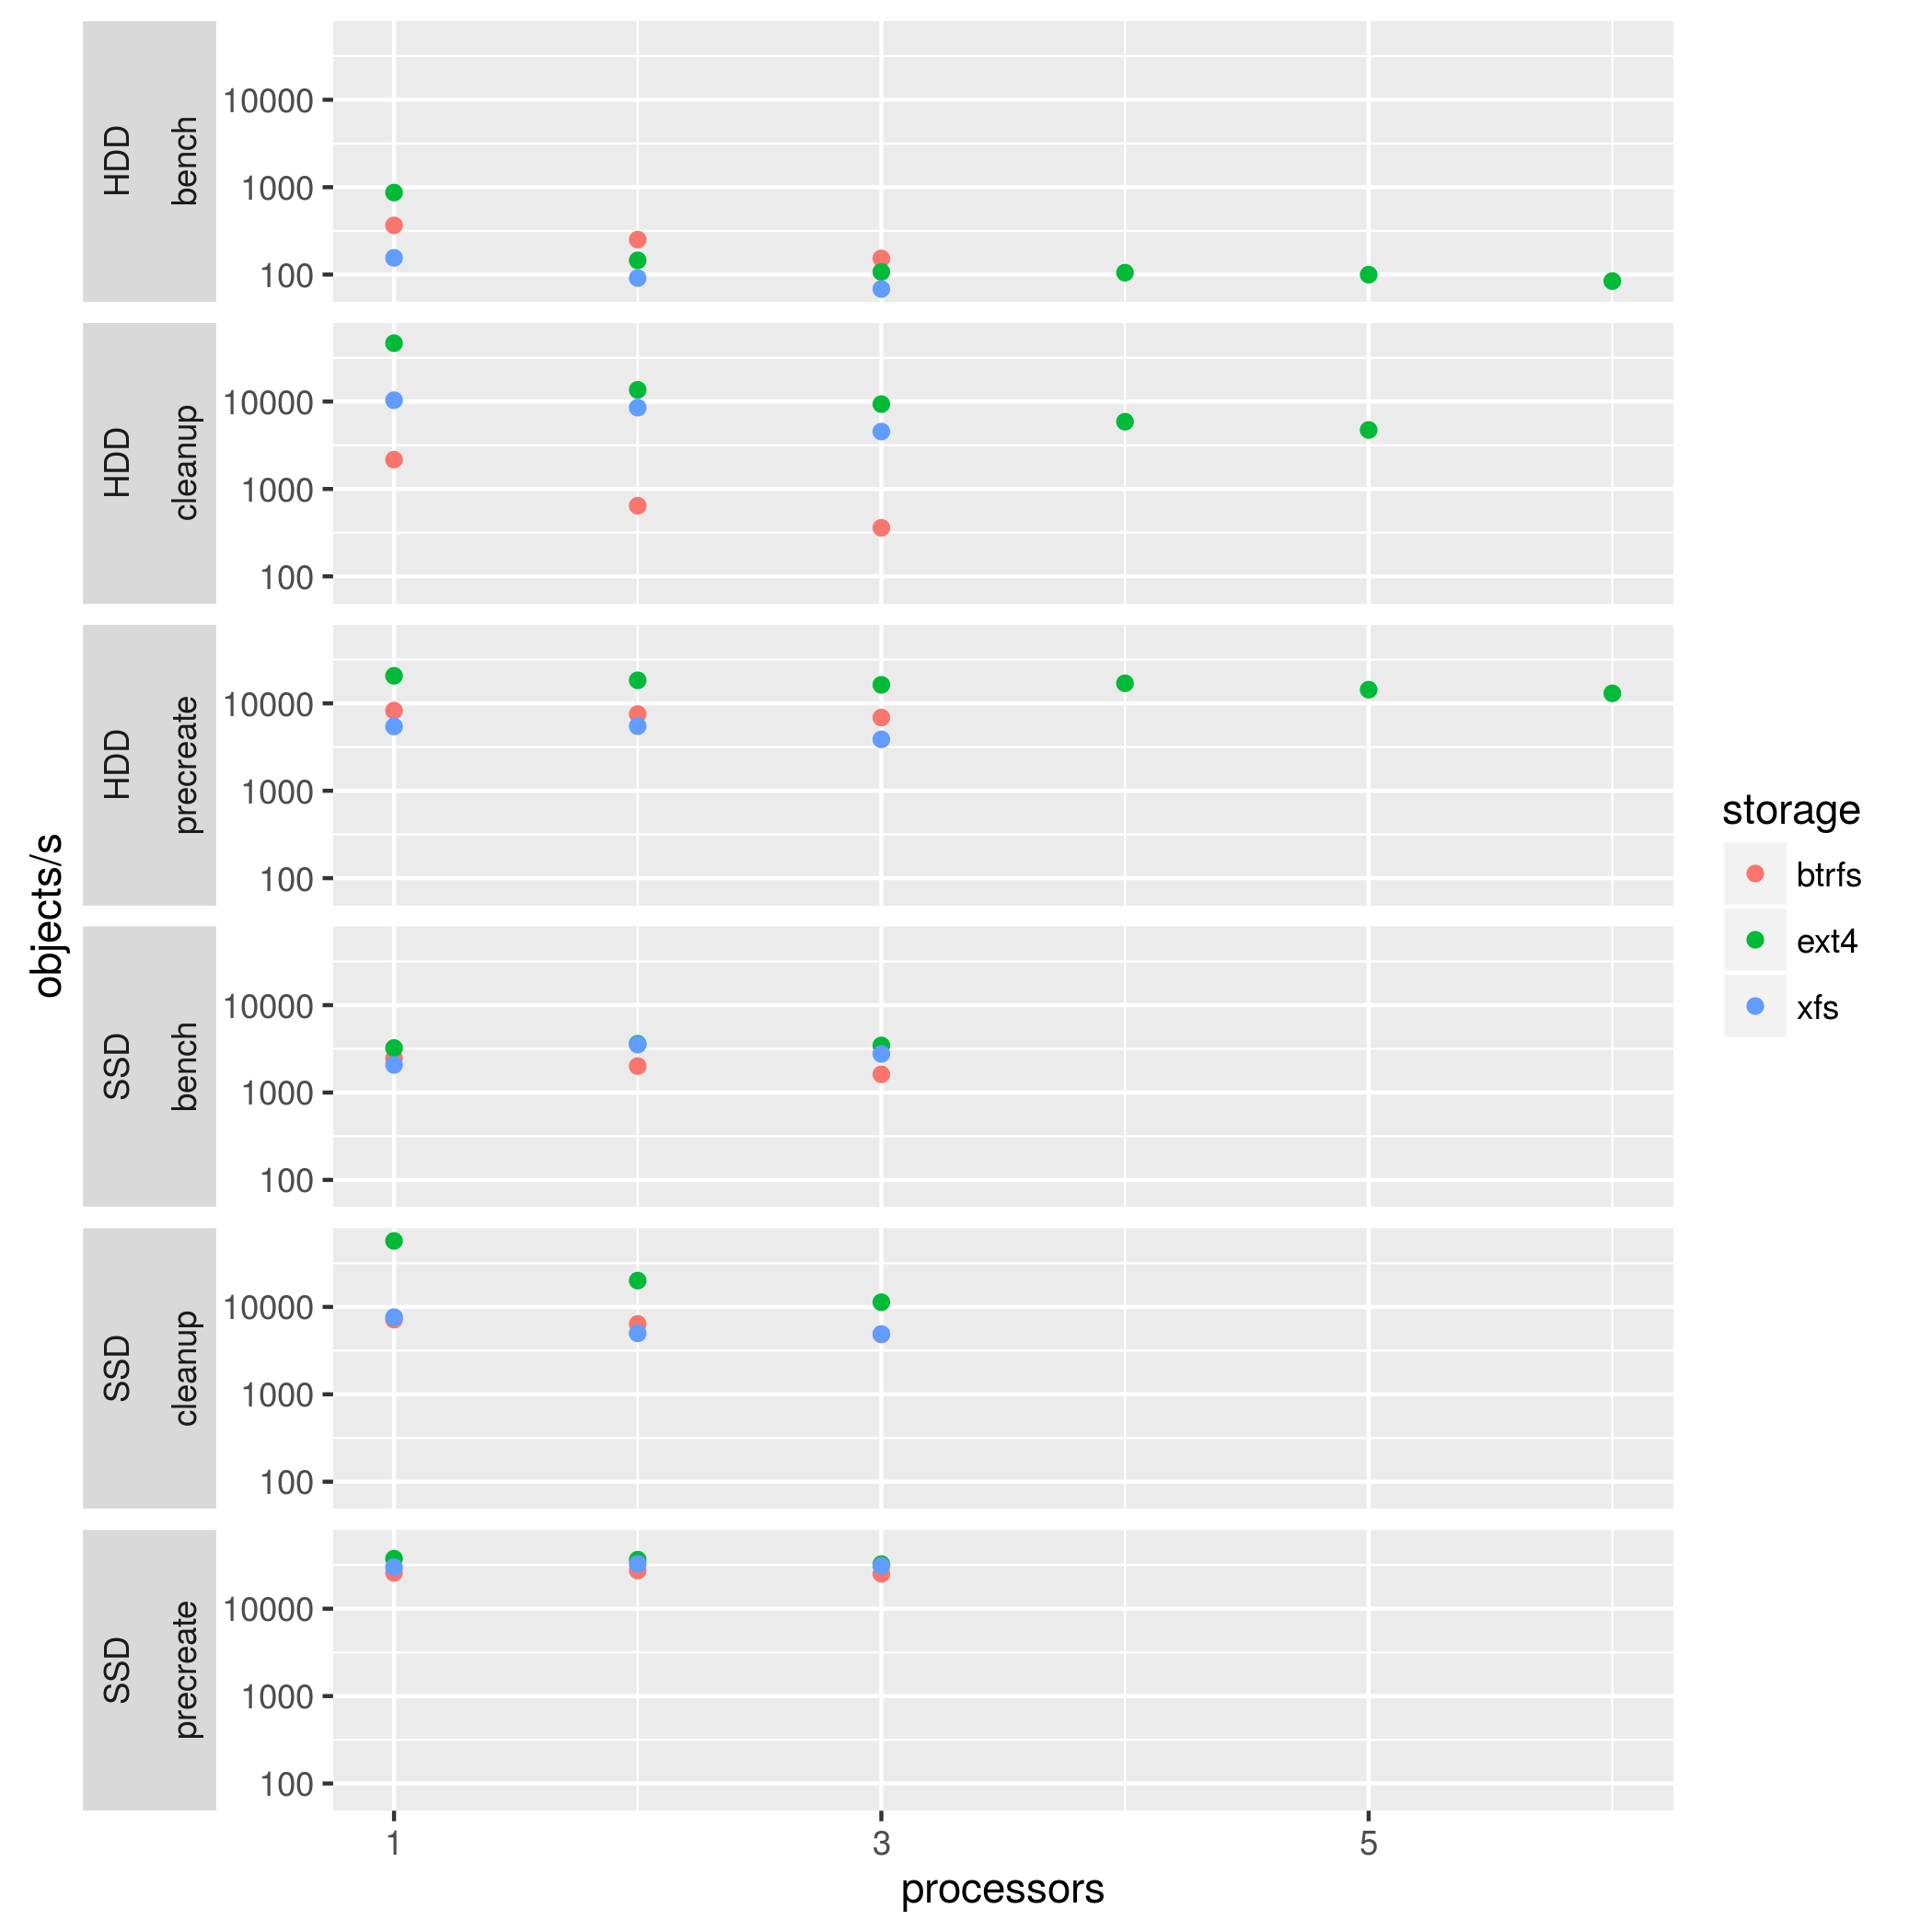
\includegraphics[width=8cm]{50tp-phases-1000Memory}}
\subfloat[]{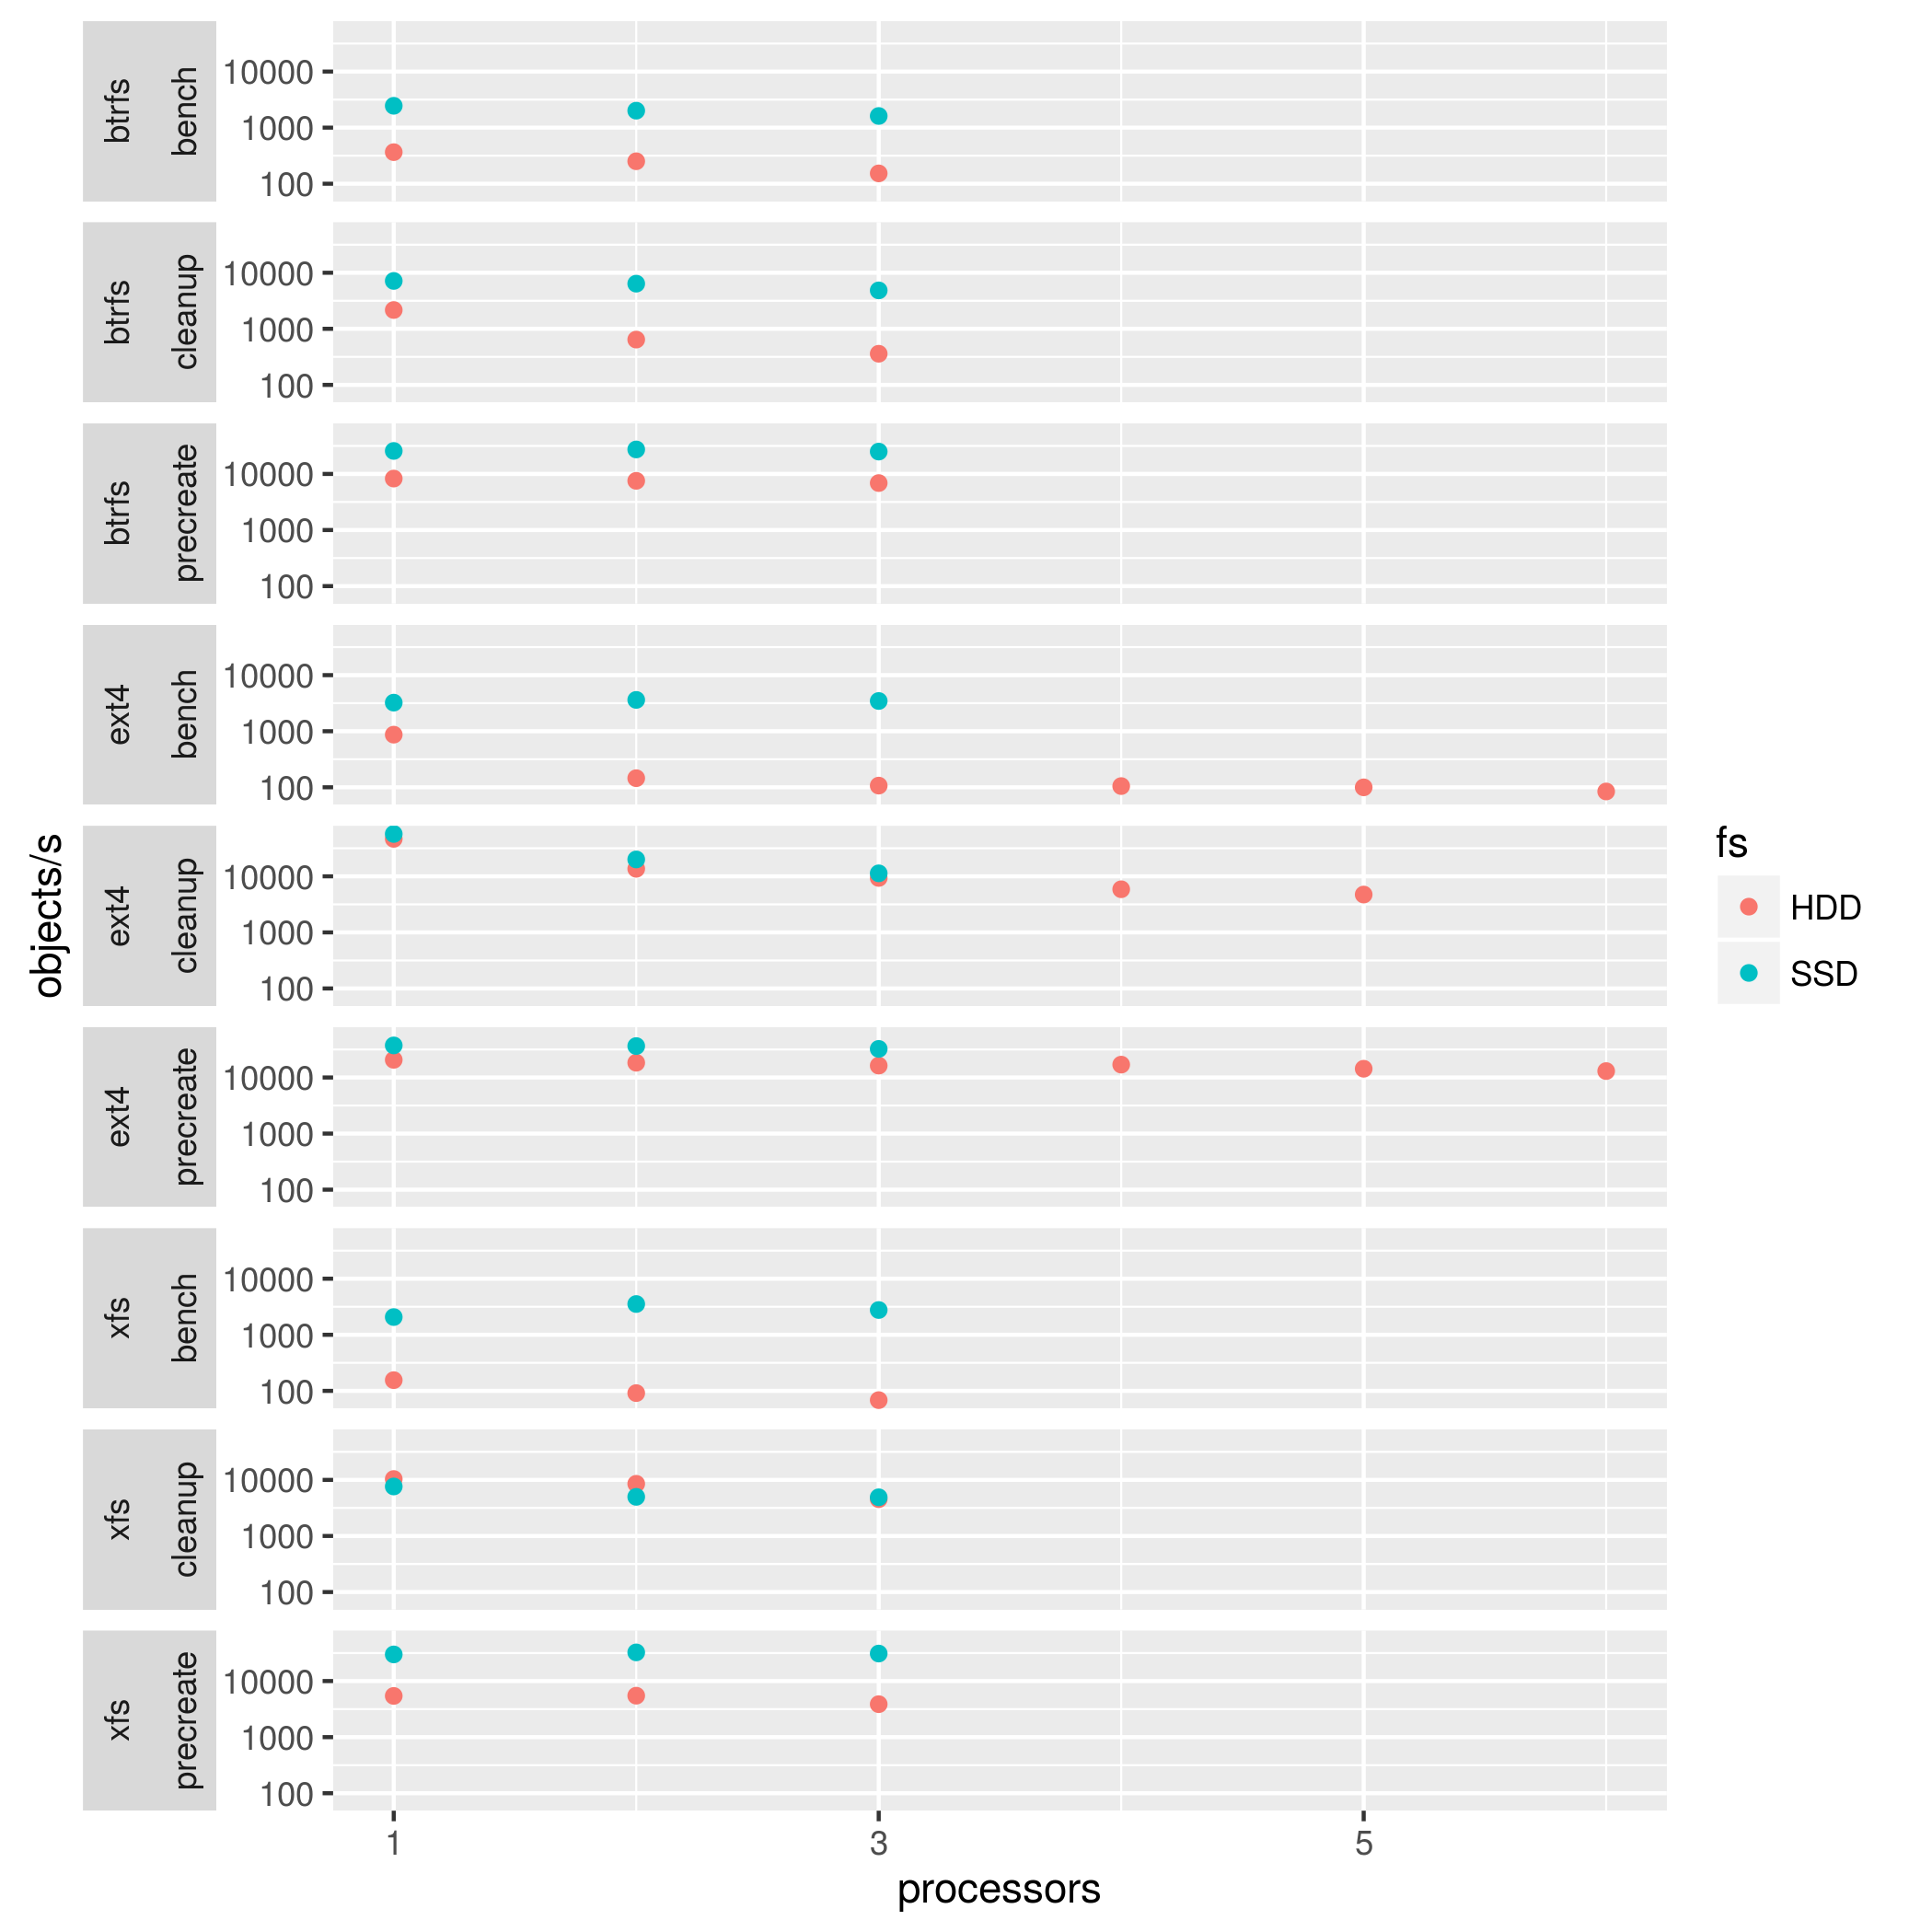
\includegraphics[width=8cm]{50tp-phases-by-storage-1000Memory}}
\caption{Results for the fixed count experiment. The y-axis uses logarithmic scale. \label{fig:fixed-count}}
\end{figure}

\paragraph{Observations:}

\begin{itemize}
\item The performance of pre-create and cleanup does not degrade much with an increase in processes and is around 10,000 ops/s.
\item HDD/bench: For the HDD, the performance of the benchmark phase is below 1000 ops/s and degrades rapidly with additional processes. 
Note that the HDD latency is around 7\,ms which leads to an expectation of roughly 150 ops/s which can be seen.
\item HDD/bench: For a single process, EXT4 dominates the other file systems with roughly 1000 ops/s, but with two and three processes, BTRFS yields better results.
\item SSD/bench: As expected, with 3,000 ops/s, the SSD delivers much better performance in this workload.
\item Comparing SSD and HDD, it can be seen that the bulk optimization for file systems leads to comparable results for precreate and cleanup phase for EXT4 and XFS.
\item The benchmarking phase shows the clear difference between the technology. 
While EXT4 and BTRFS can optimize the access pattern for one process, the performance on HDD quickly degrades with multiple processes.
\end{itemize}

\paragraph{Variability:}
The variability of the different repeated measurements within one run is briefly discussed next.
\Cref{fig:variability} shows the individual measurements for the 5 repeats for the benchmark phase on one and two processors.
For the SSD, it can be seen that there is some variability but overall performance is stable.
For the HDD, the first iteration yields different results for BTRFS and XFS than the next iterations.
With two processes, the first iteration does not differ too much.
For EXT4, this might be caused from the fact that with one process, the directories are accessed at the same position and, since previously created files are read, 50 read and 50 write “streams” are needed.
Since metadata and data is placed together, it could be pre-fetched and available on the HDD read cache. 
With two processes the number increases to 100 making it impossible to utilize the cache.

\begin{figure}
\centering
\subfloat[1 process]{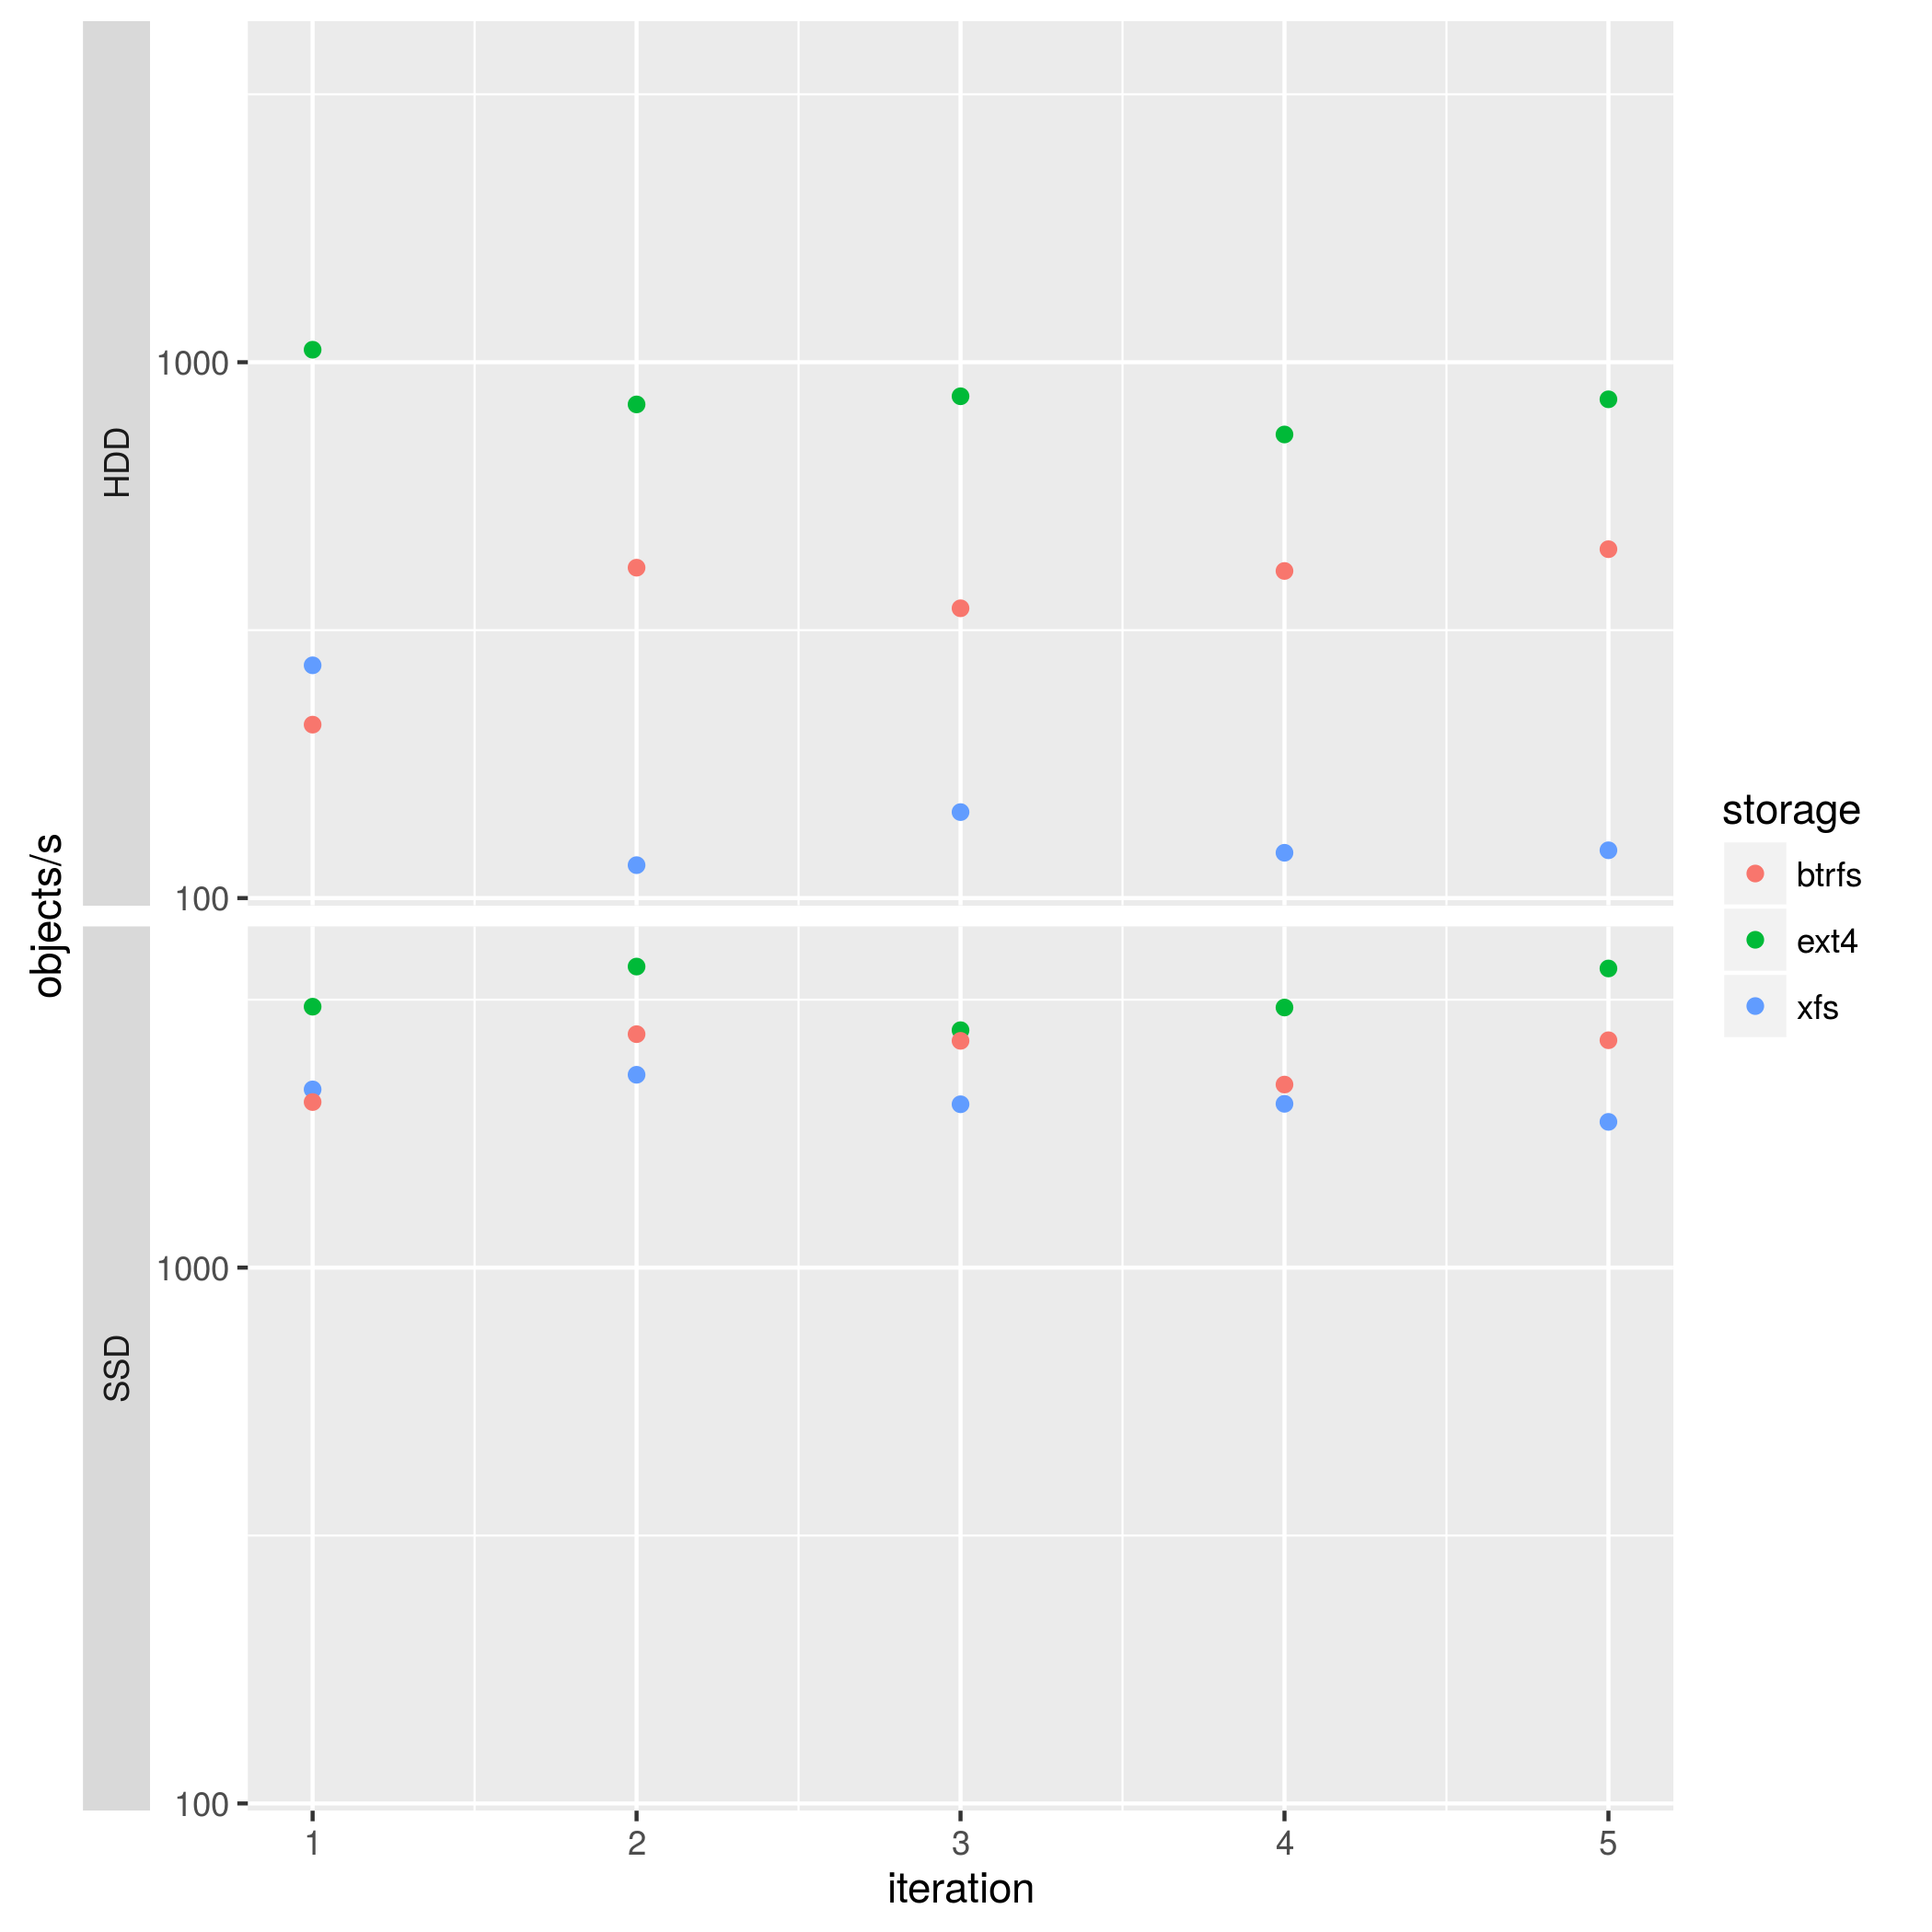
\includegraphics[width=8cm]{50tp-fs}}
\subfloat[2 processes]{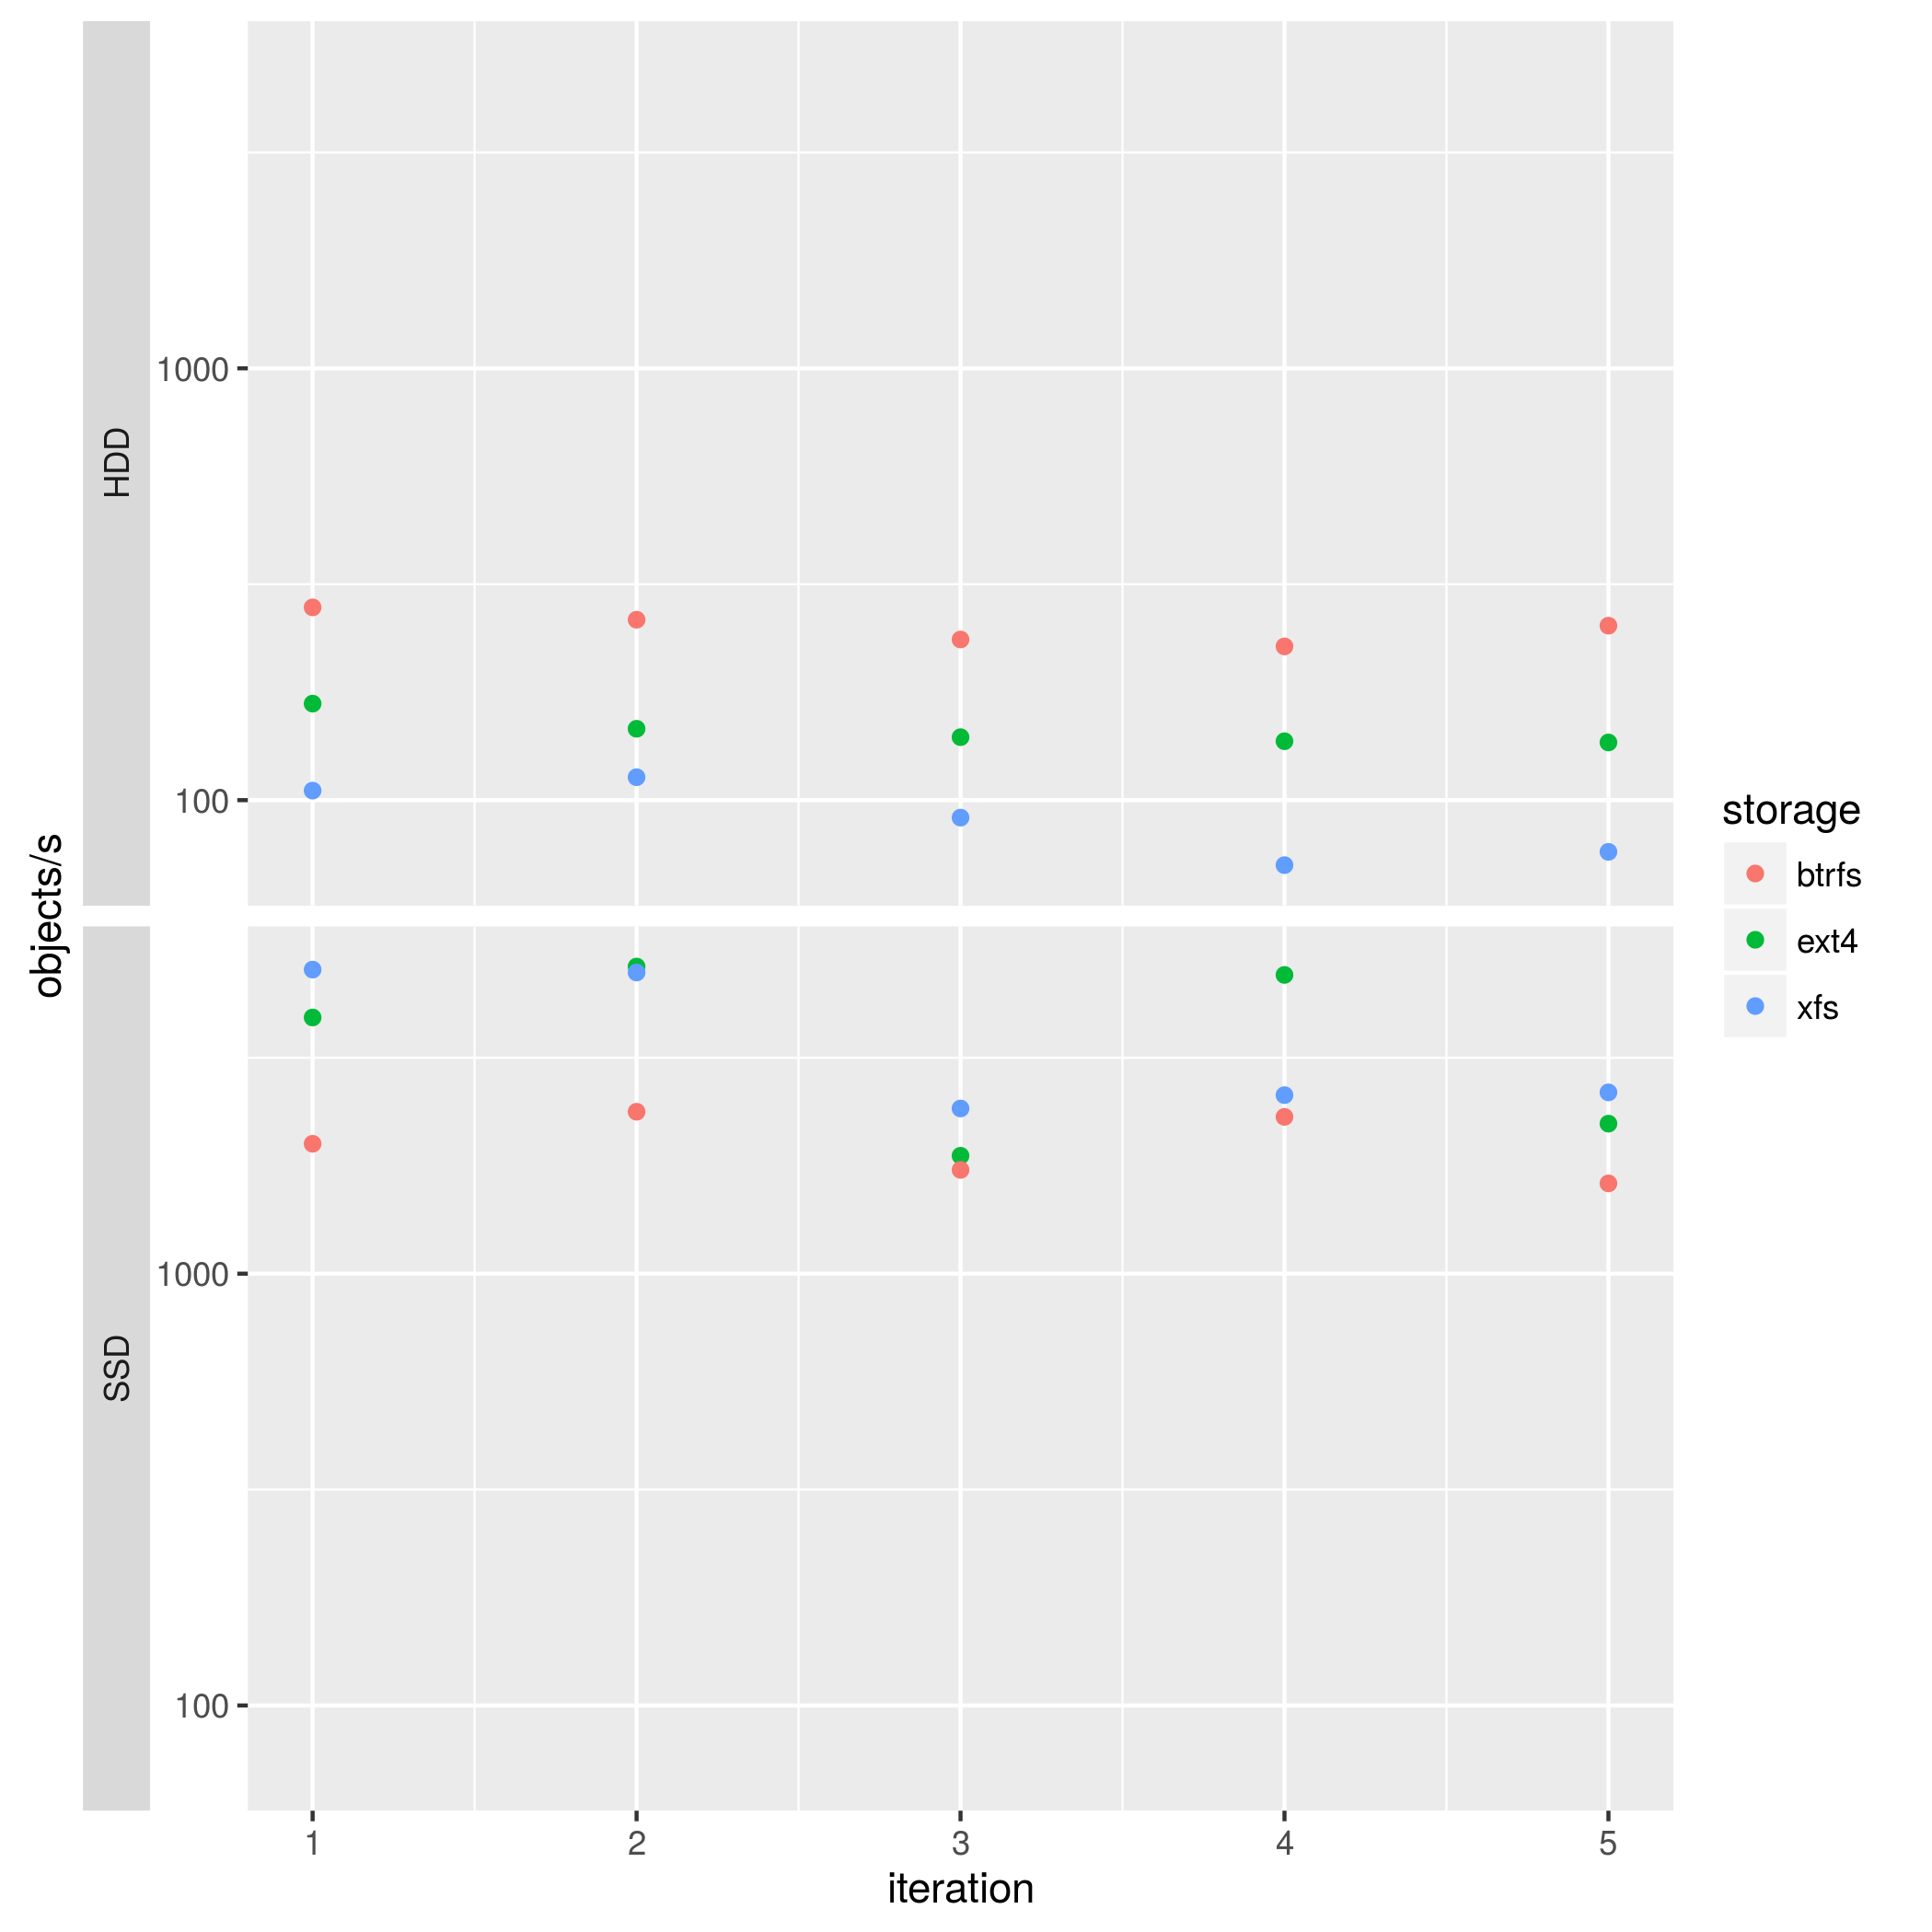
\includegraphics[width=8cm]{50tp-2proc-fs}}
\caption{Variability between the repeated runs. \label{fig:variability}}
\end{figure}



%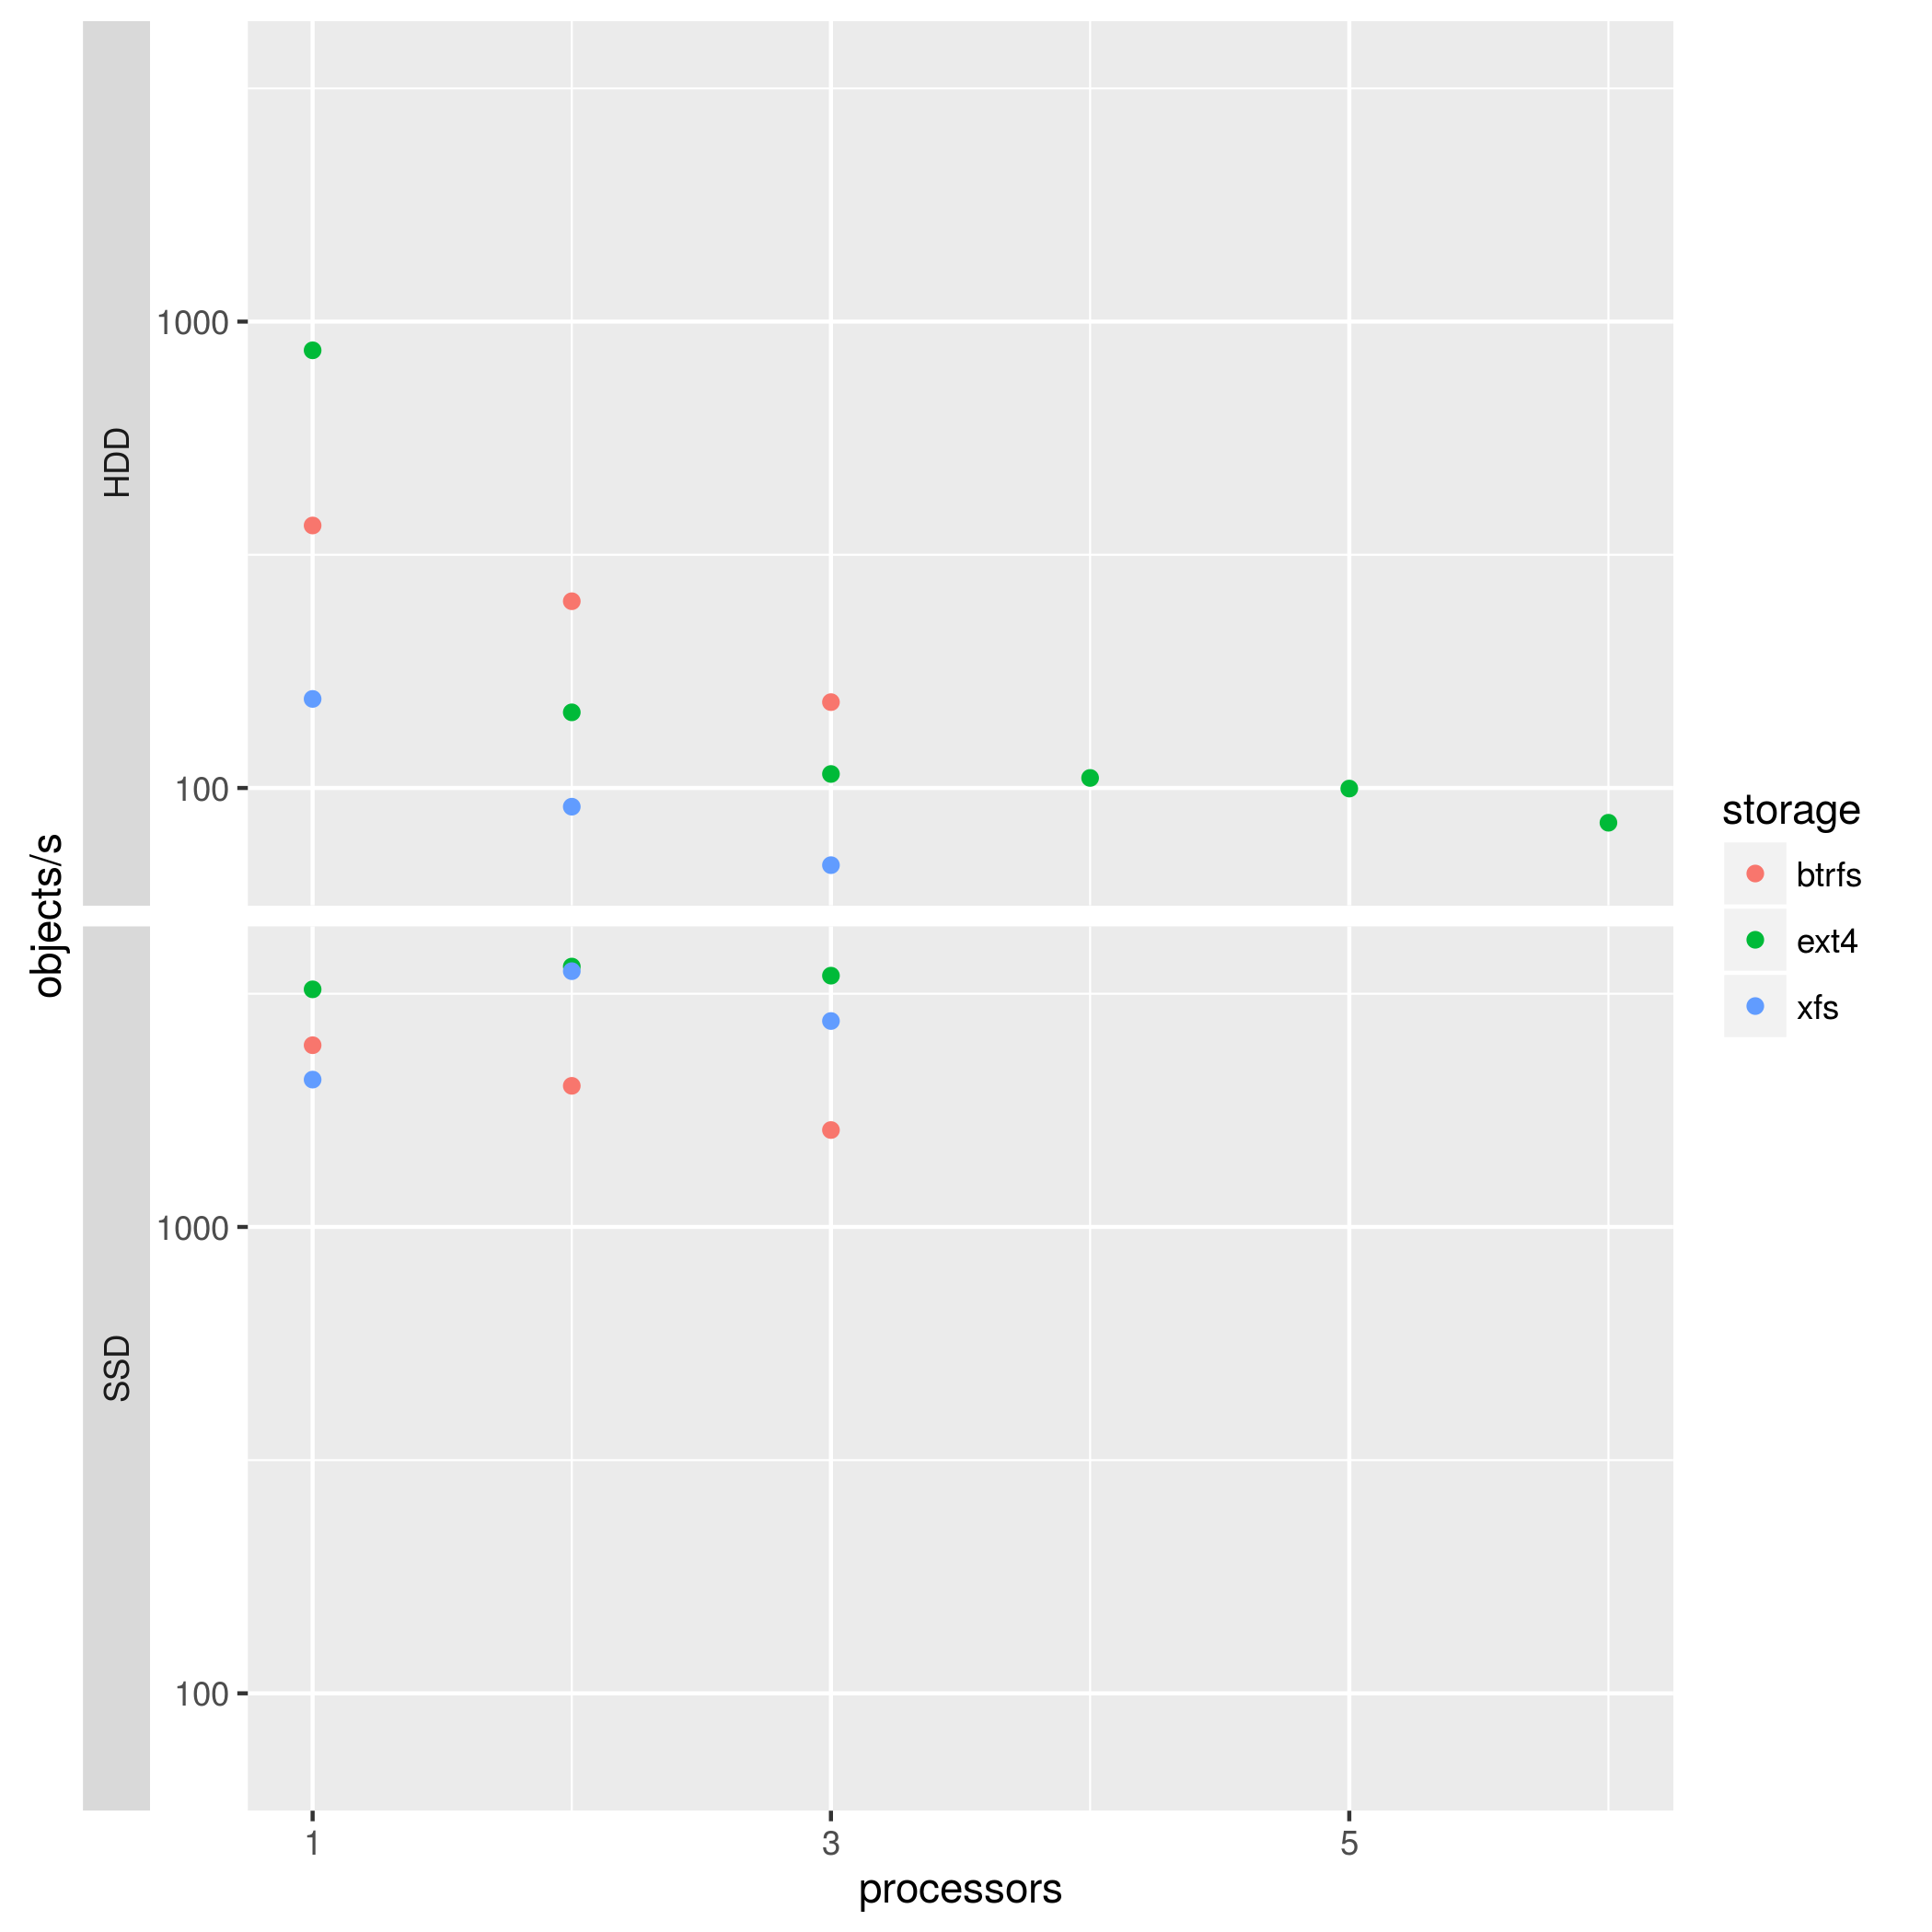
\includegraphics[width=8cm]{50tp-proc-1000Memory}
%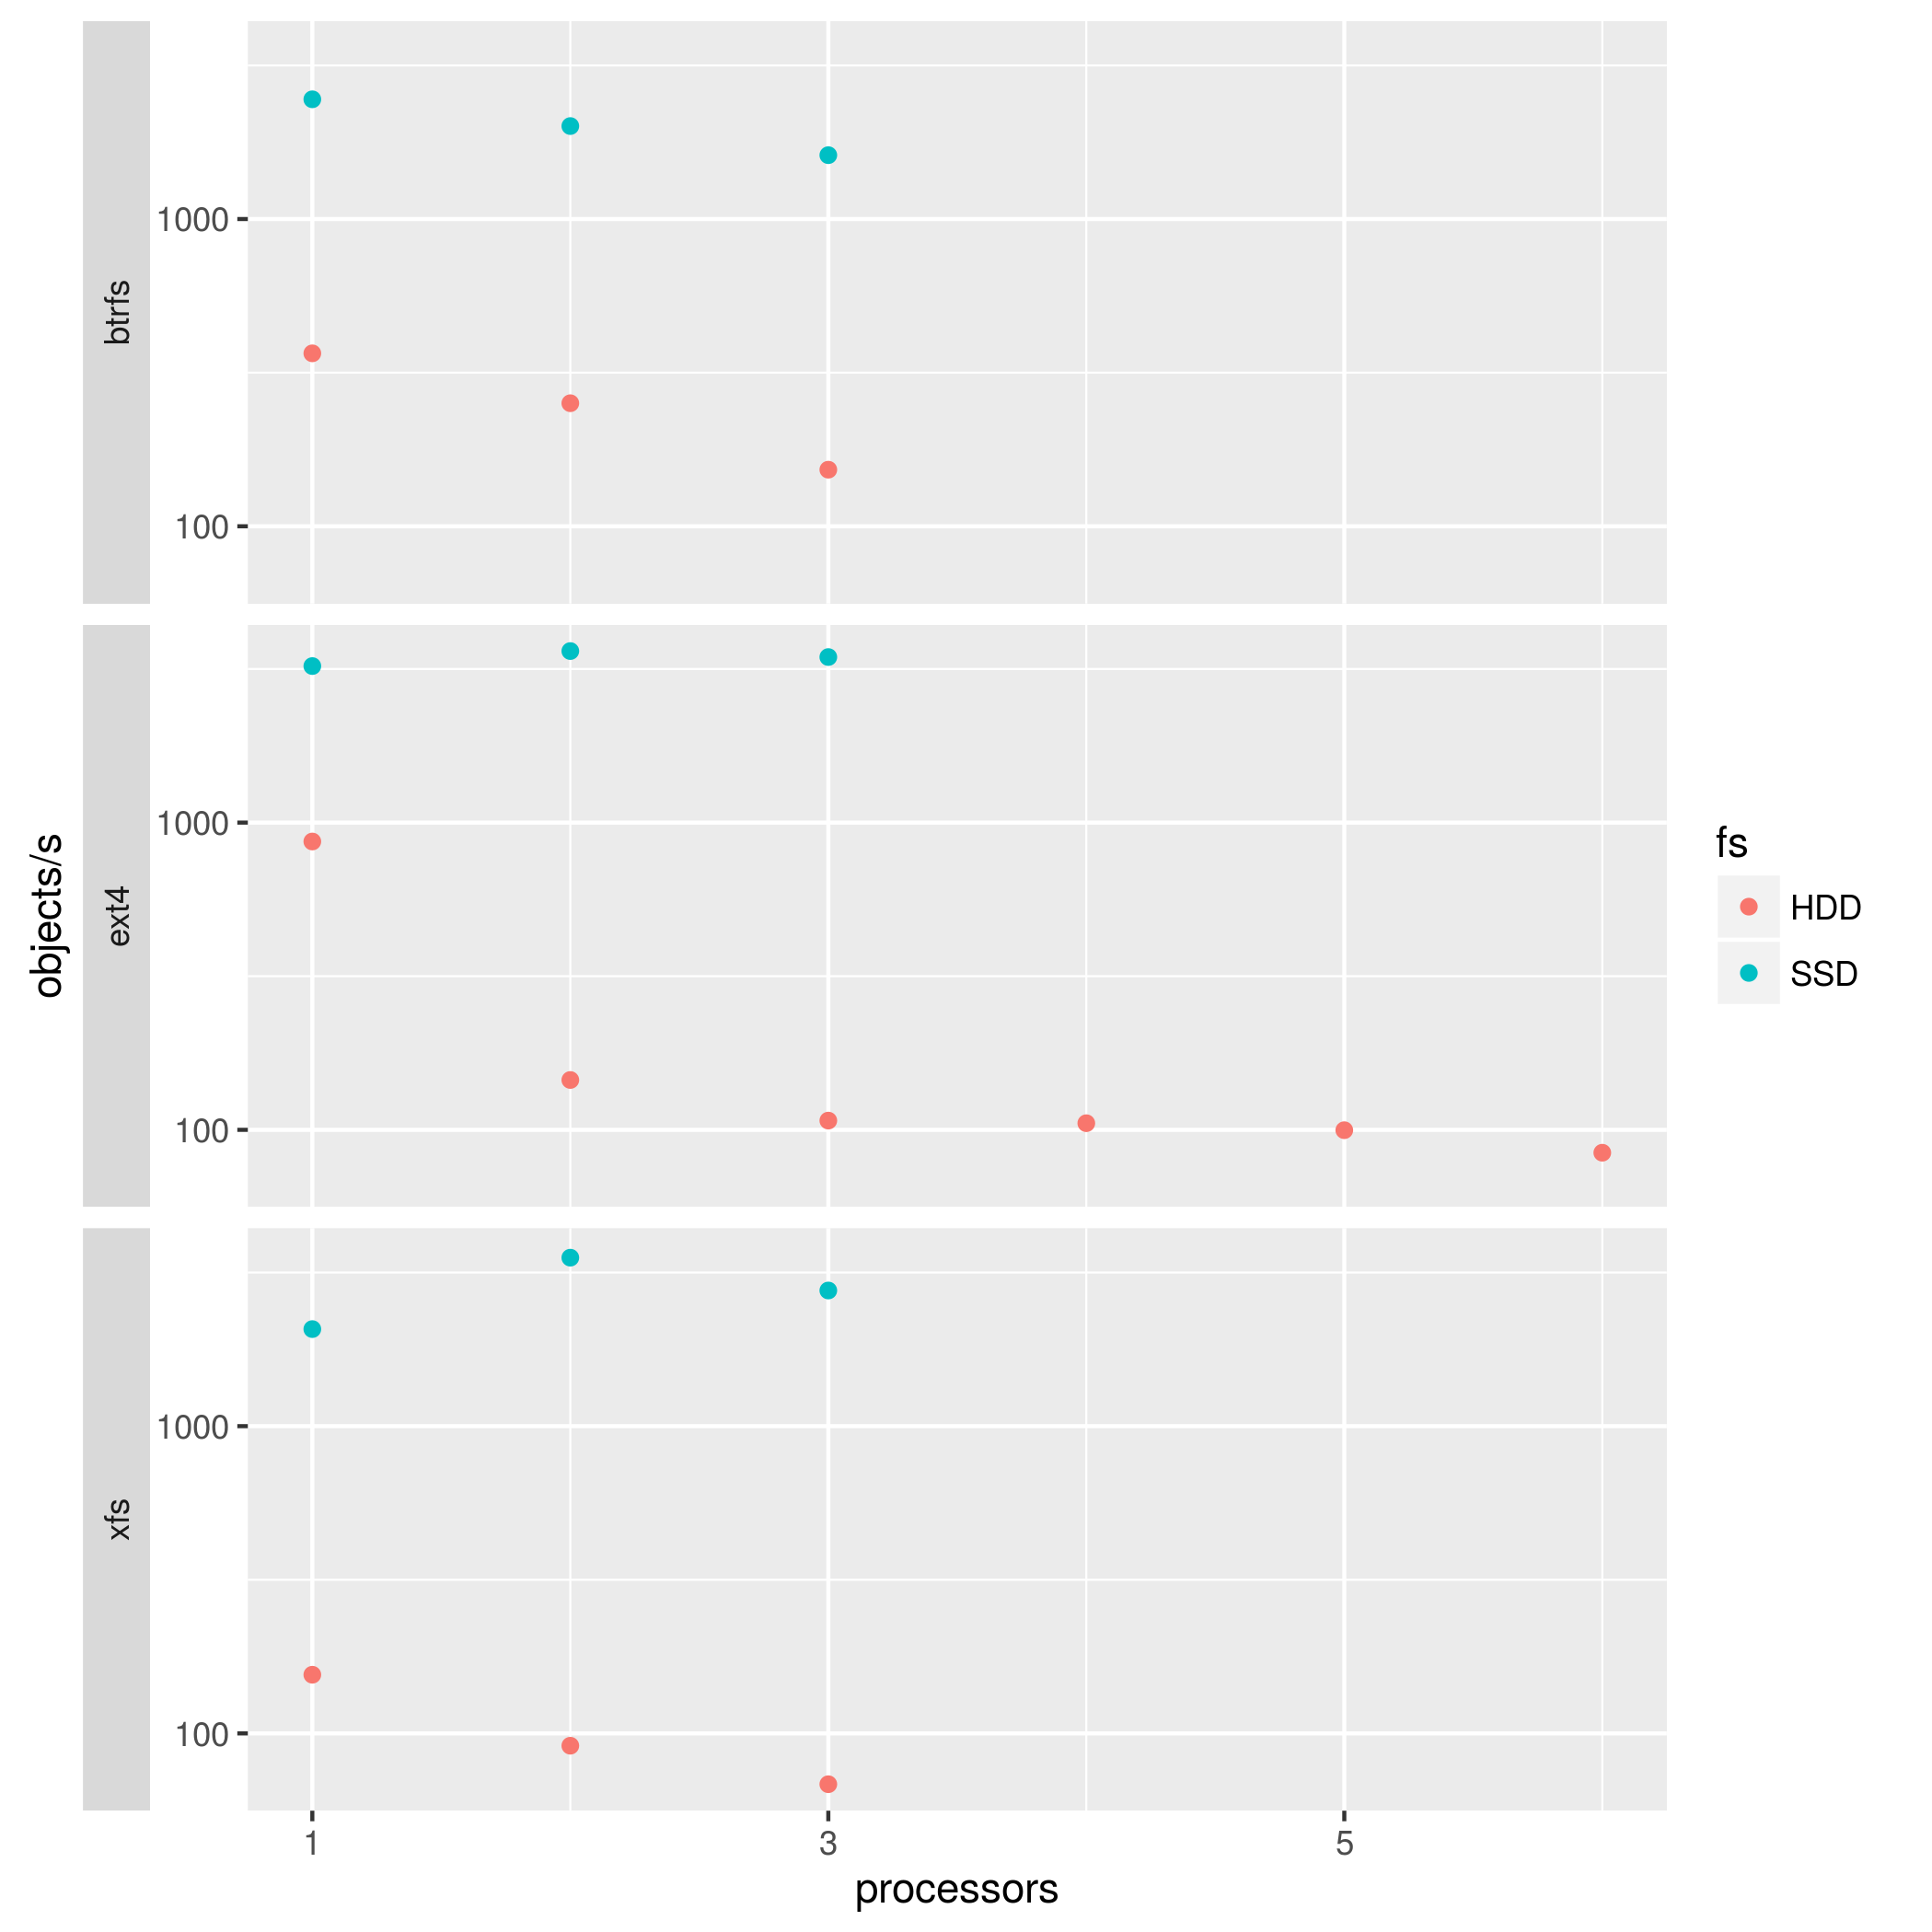
\includegraphics[width=8cm]{50tp-proc-by-storage-1000Memory}


\subsection{Results for Variable Number of Objects}

The results for our settings where the number of objects increases with each process are given in the following.
Since the working set is 110 MiB times the number of processes, this workload can be cached much better and allows to investigate caching behavior.

\Cref{fig:variable-count-u}
\Cref{fig:variable-count-1000}

\paragraph{Results:}

\begin{figure}
\centering
\subfloat[]{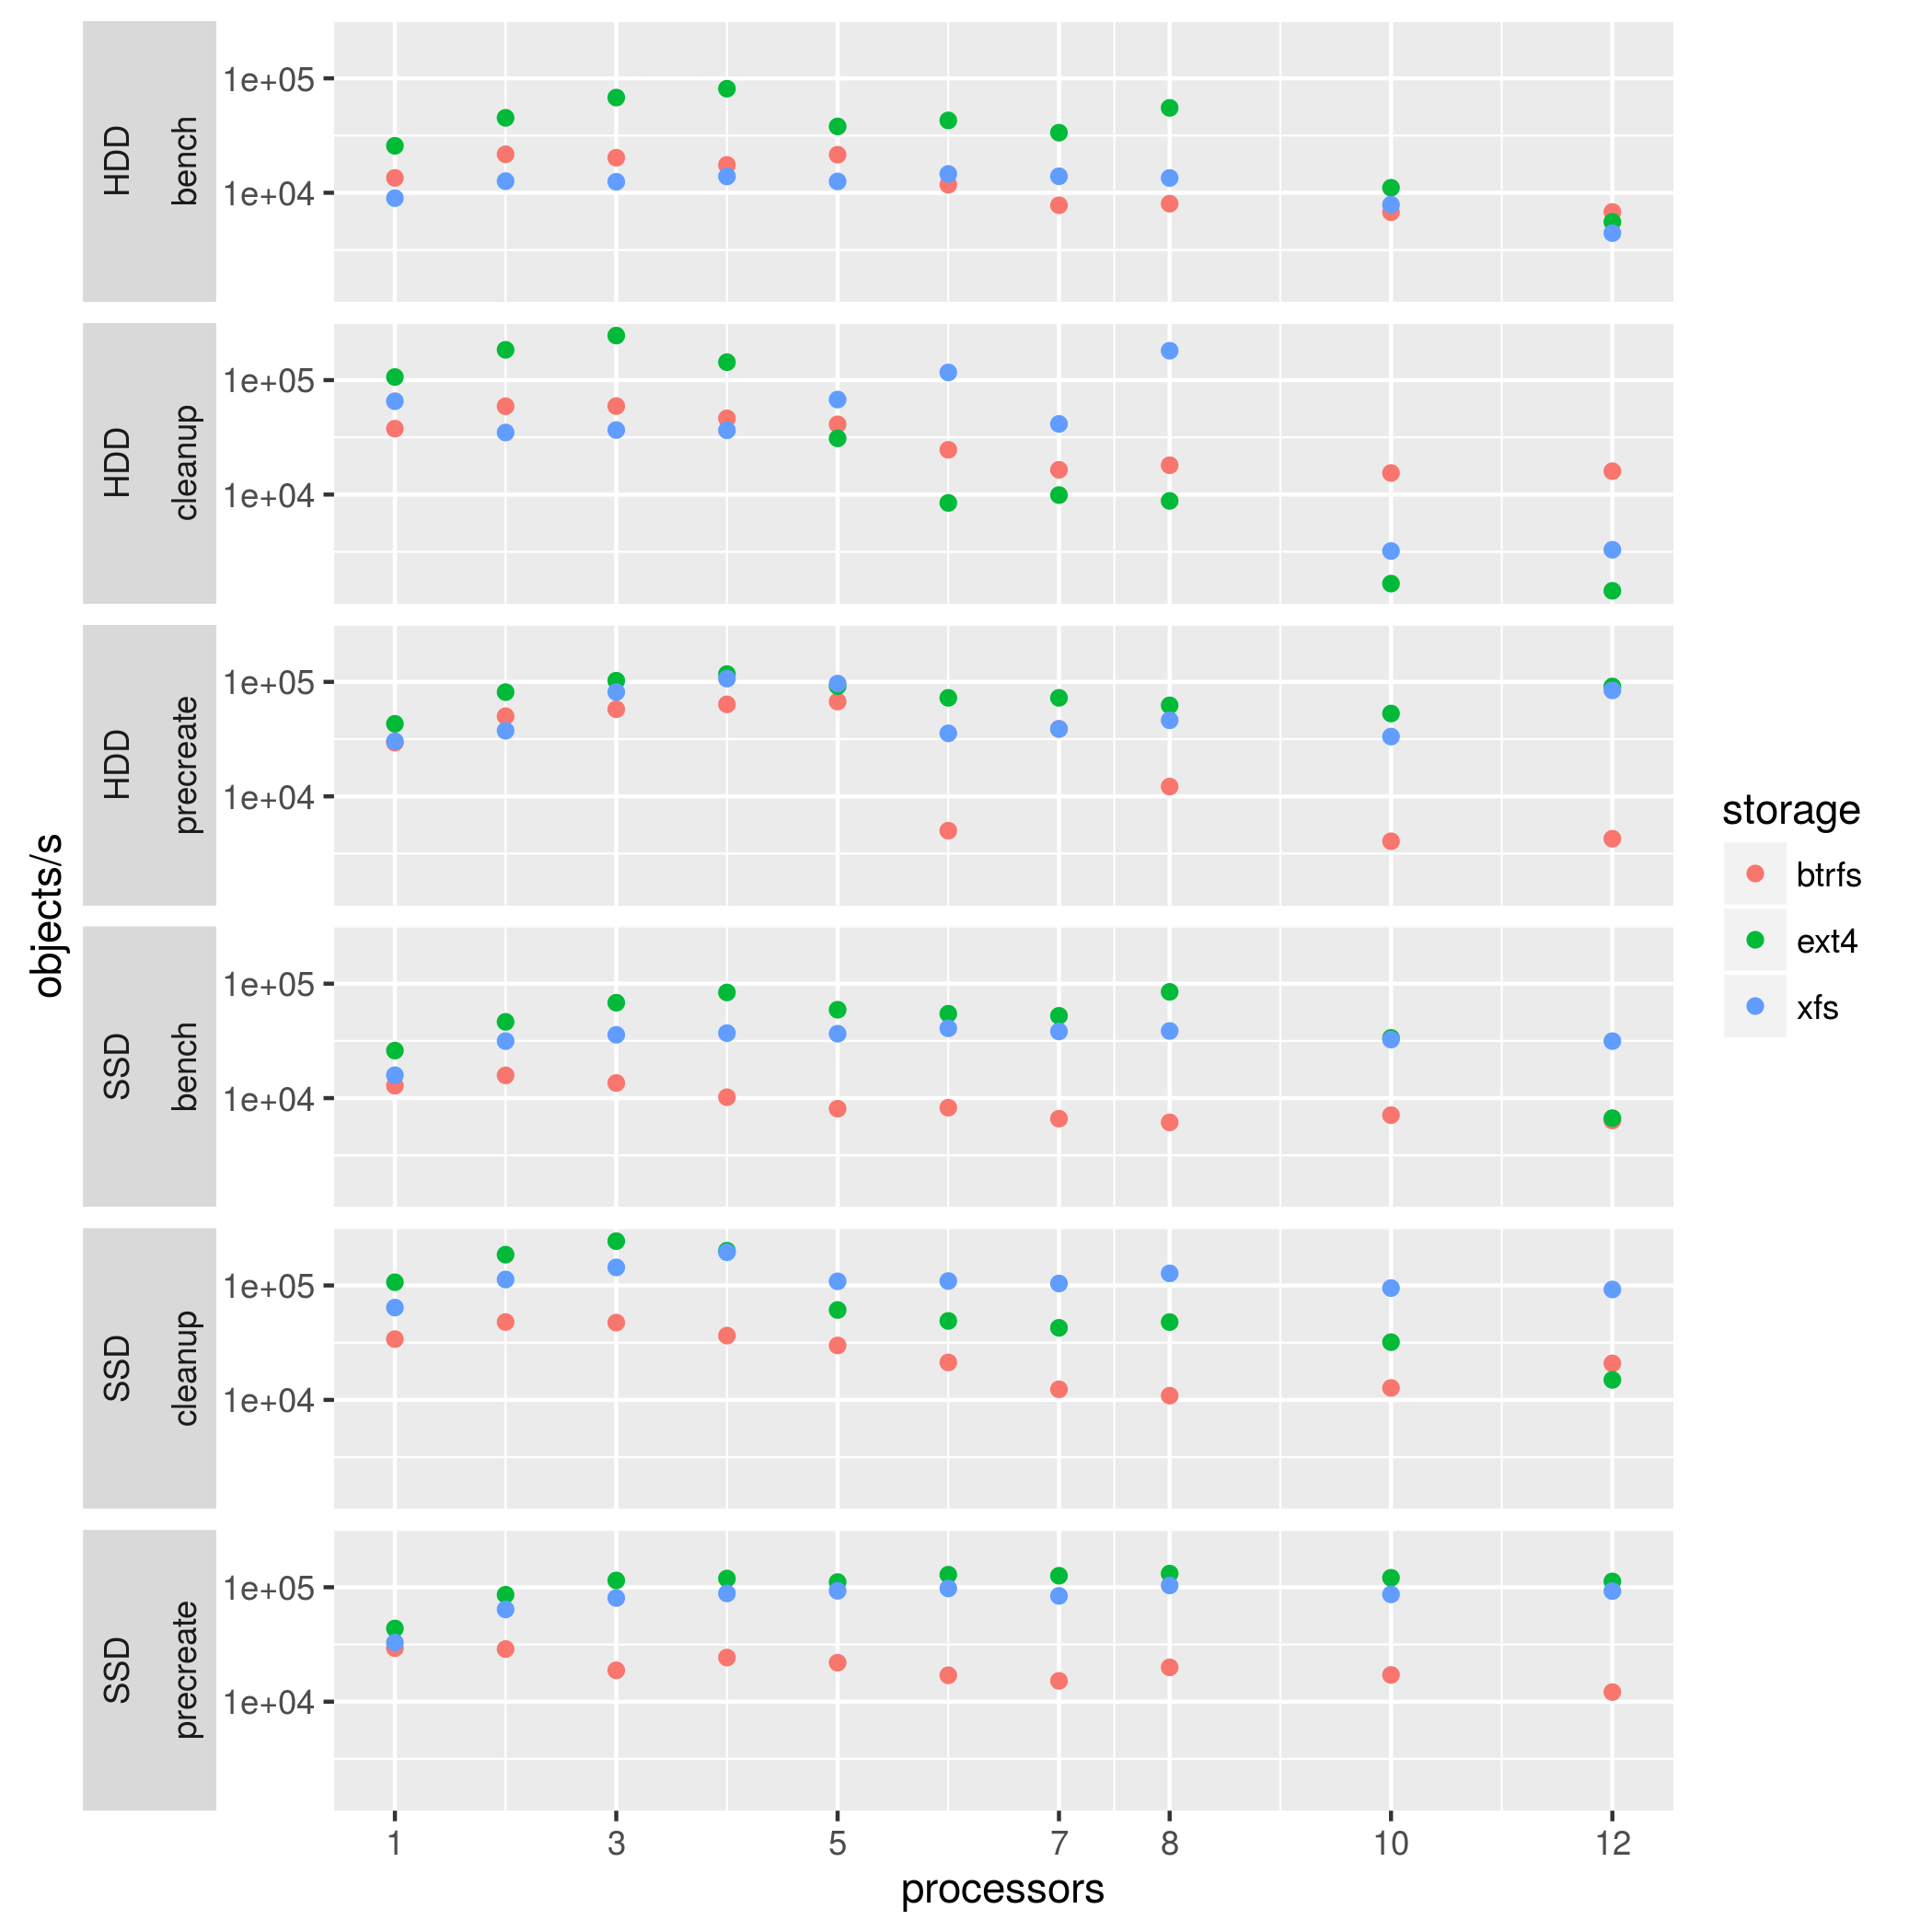
\includegraphics[width=8cm]{tp-phase-unlimitedMemory}}
\subfloat[]{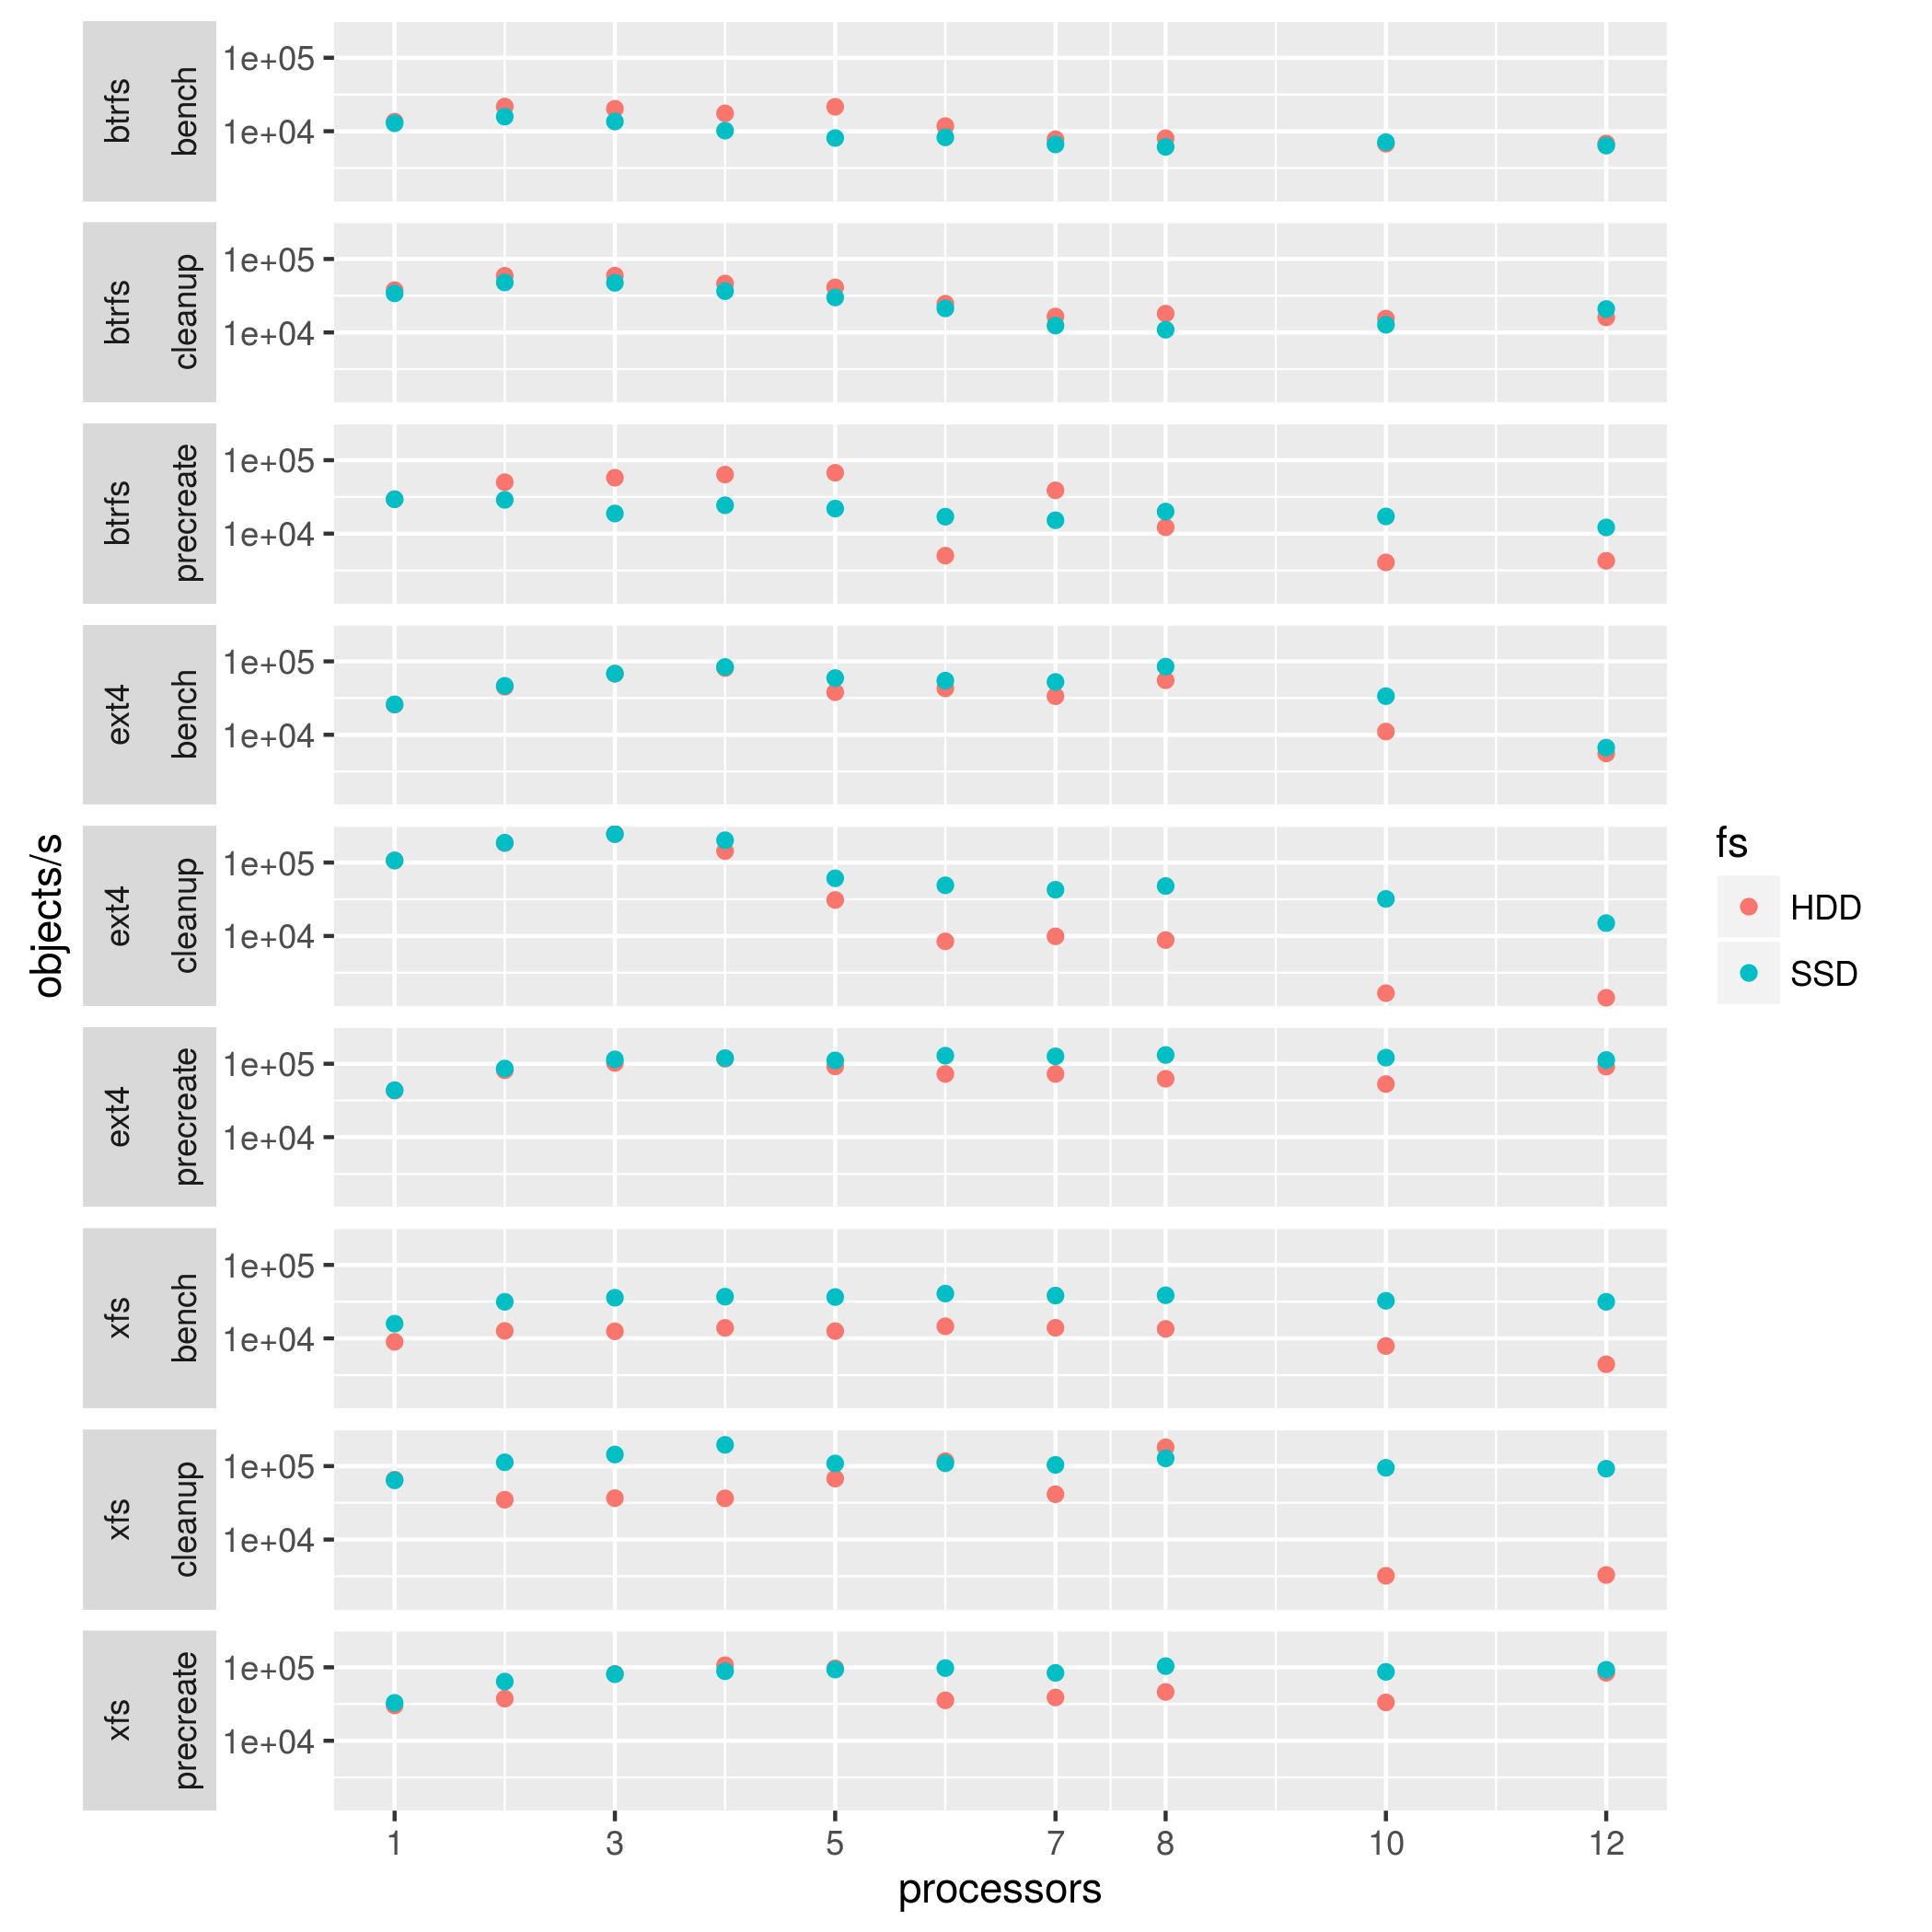
\includegraphics[width=8cm]{tp-phase-by-storage-unlimitedMemory}}
\caption{Results for the variable n experiment with unlimited memory. The y-axis uses logarithmic scale. \label{fig:variable-count-u}}
\end{figure}


\begin{figure}
\centering
\subfloat[]{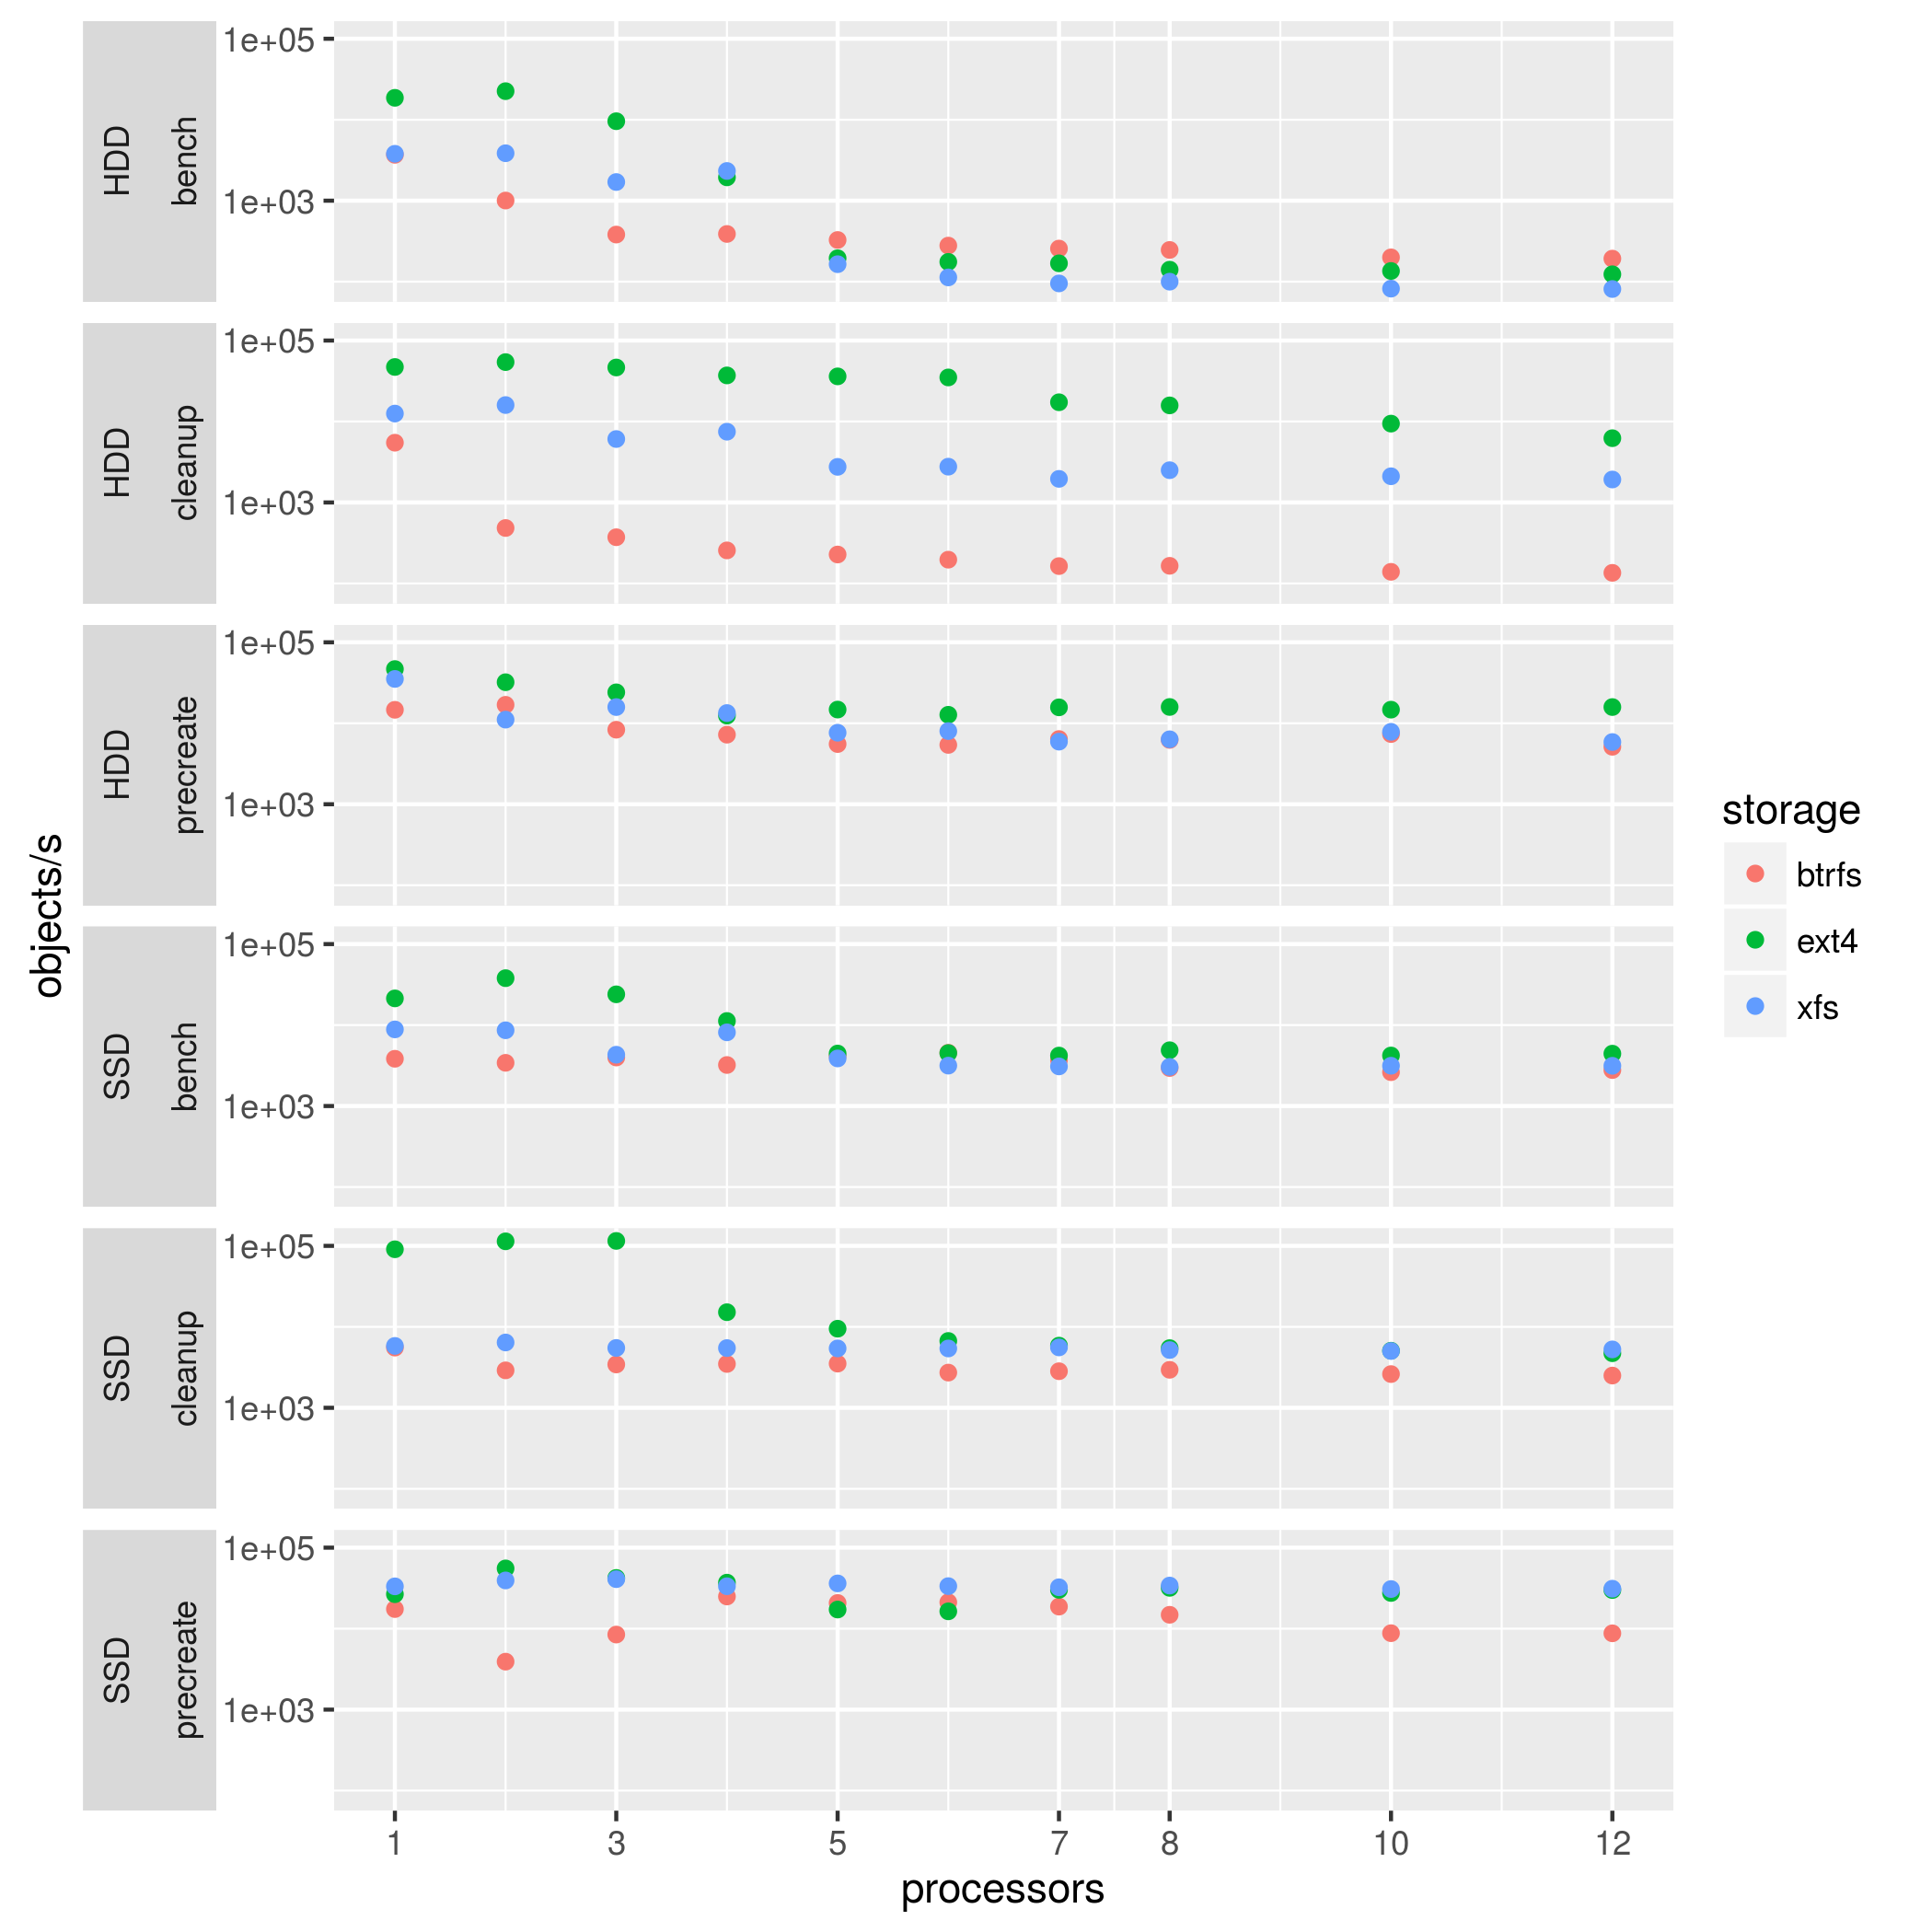
\includegraphics[width=8cm]{10tp-phases-1000Memory}}
\subfloat[]{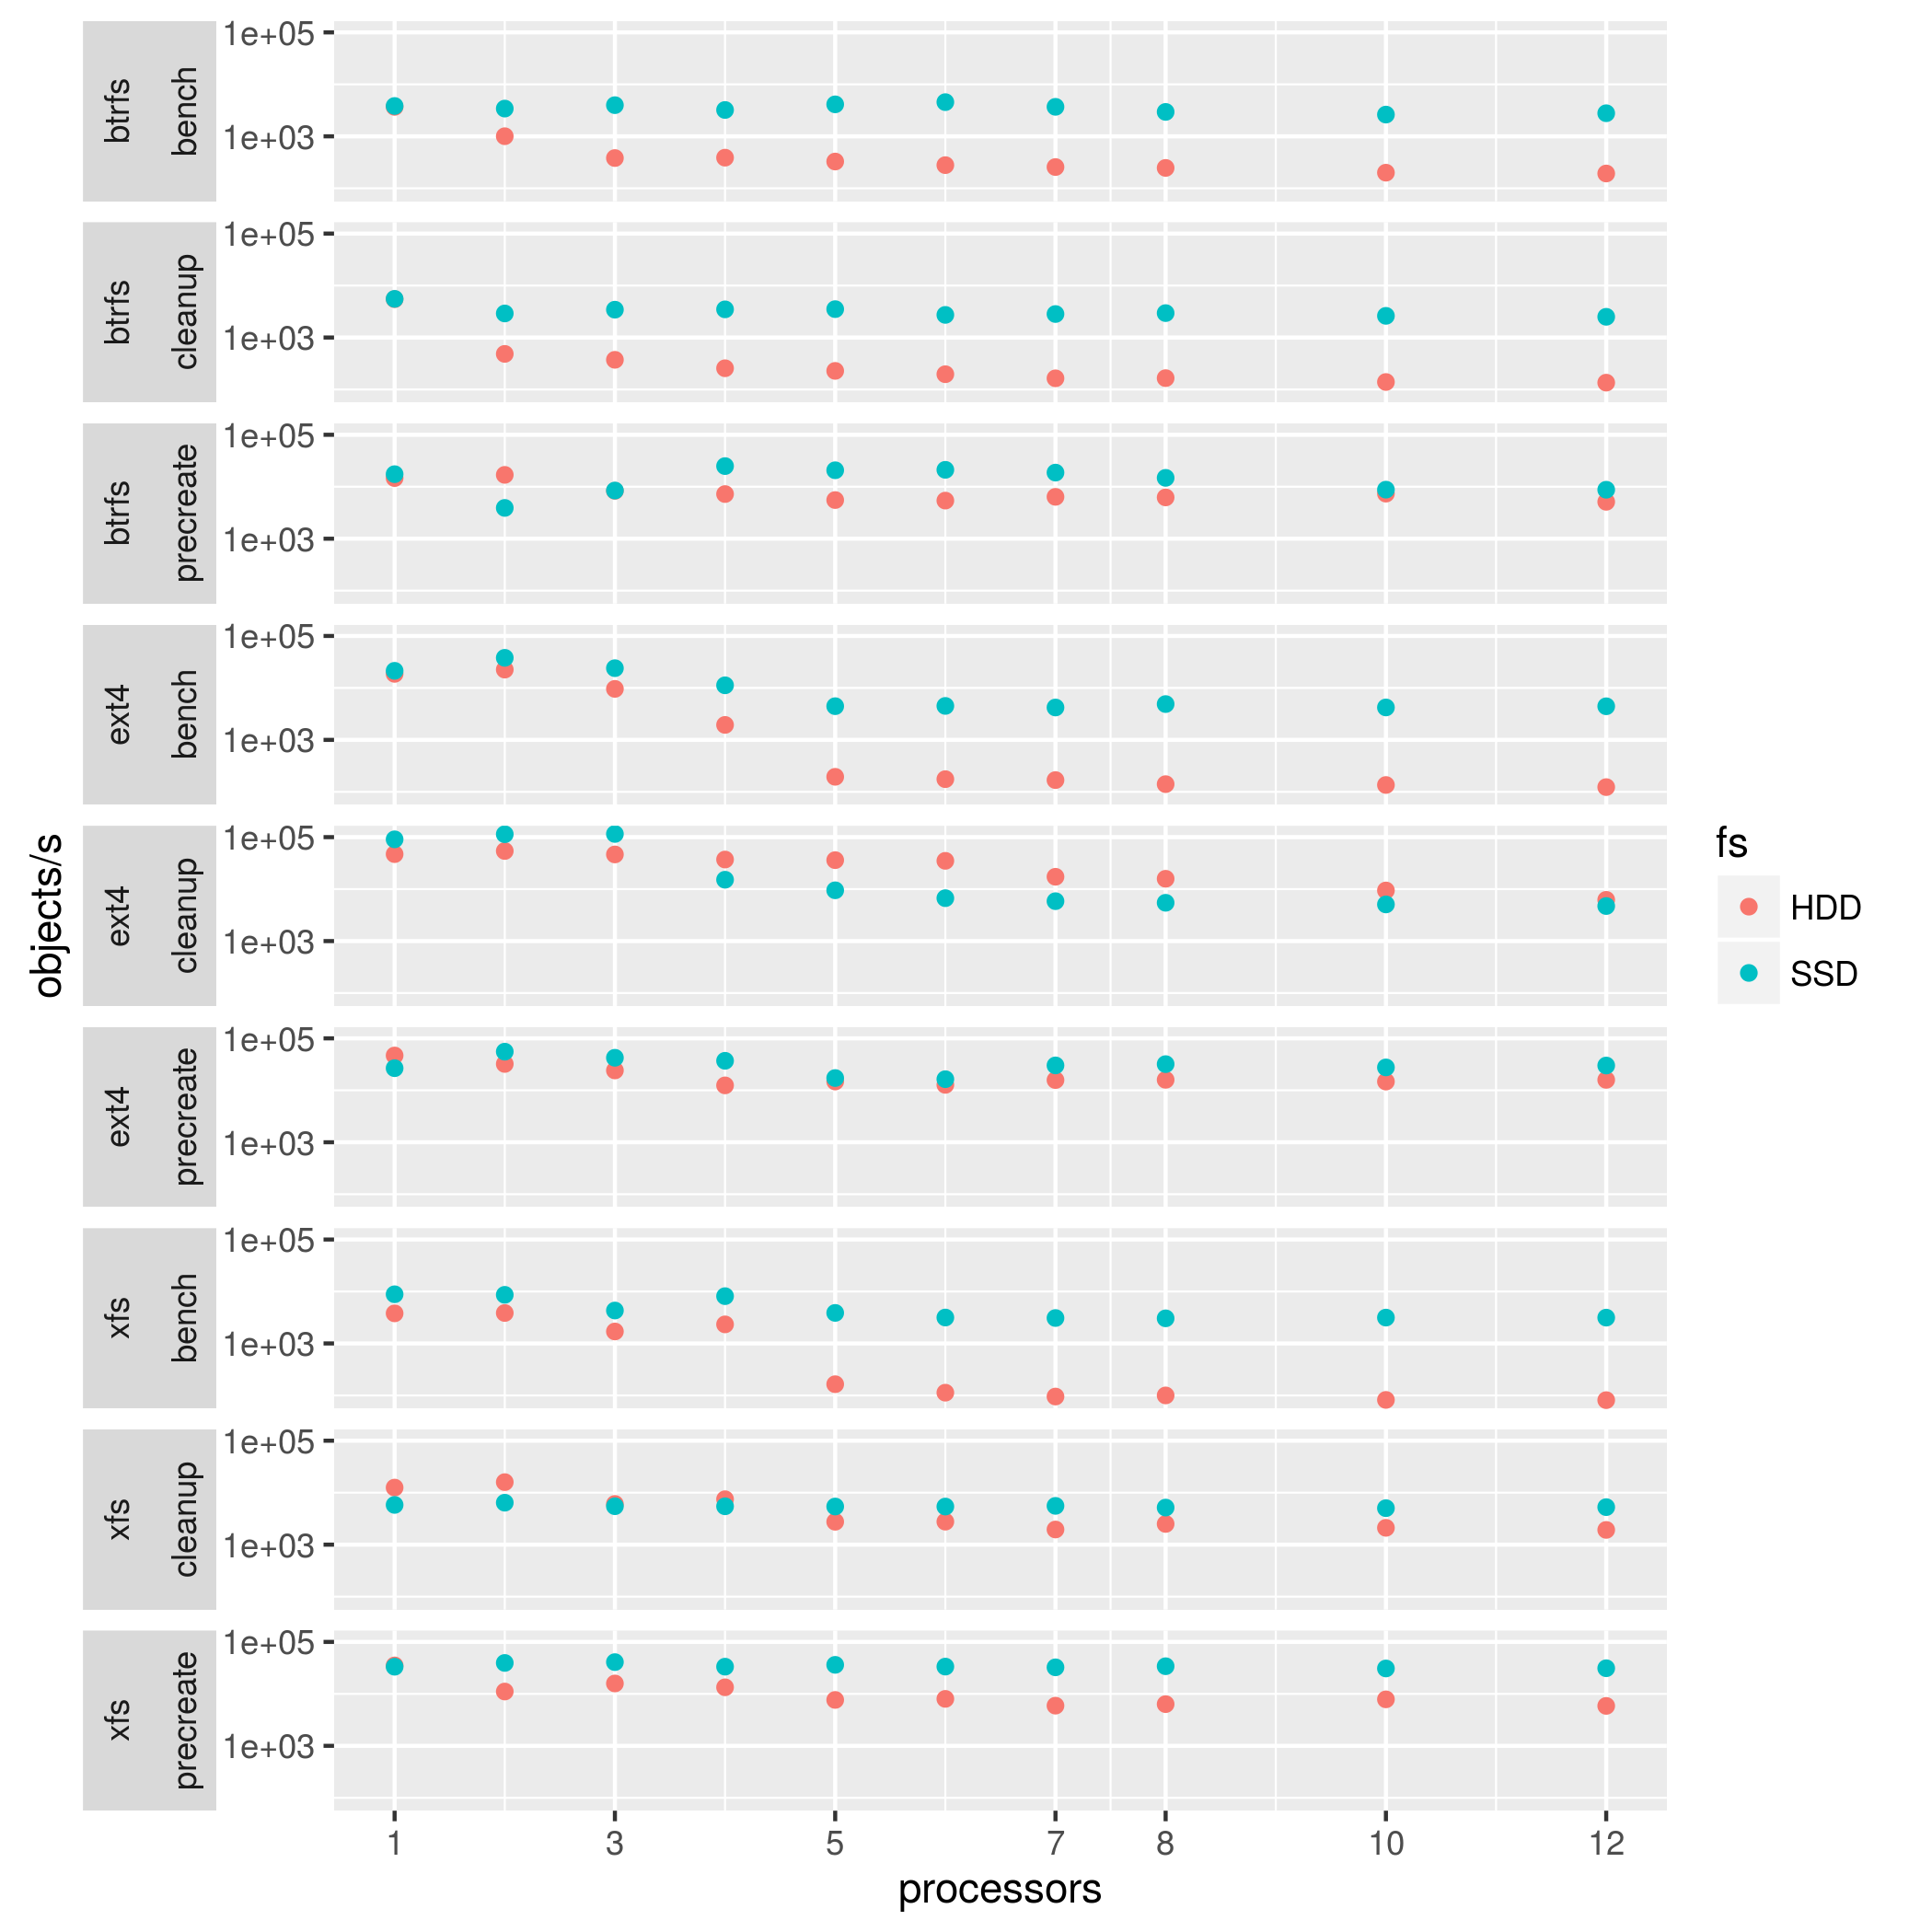
\includegraphics[width=8cm]{10tp-phases-by-storage-1000Memory}}
\caption{Results for the variable n experiment with 1000 MB free memory. The y-axis uses logarithmic scale. \label{fig:variable-count-1000}}
\end{figure}



\paragraph{Variability:}
The variability of the different repeated measurements within one run is briefly discussed next.
\Cref{fig:10variability} shows the individual measurements for the 5 repeats for the benchmark phase on one and two processors.
Since the amount of data is cacheable, naturally, the results vary more.
Now, all file systems behave slightly different on the first iteration, than on the others.
With two processes, the first iteration does not differ too much, but on the example on BTRFS we can observe that different repeats may lead to totally different performance numbers (100 ops/s vs. 2000 ops/s in Iteration 2 and 4).
The value depends on the internal write-back cycle.

\begin{figure}
\centering
\subfloat[1 process]{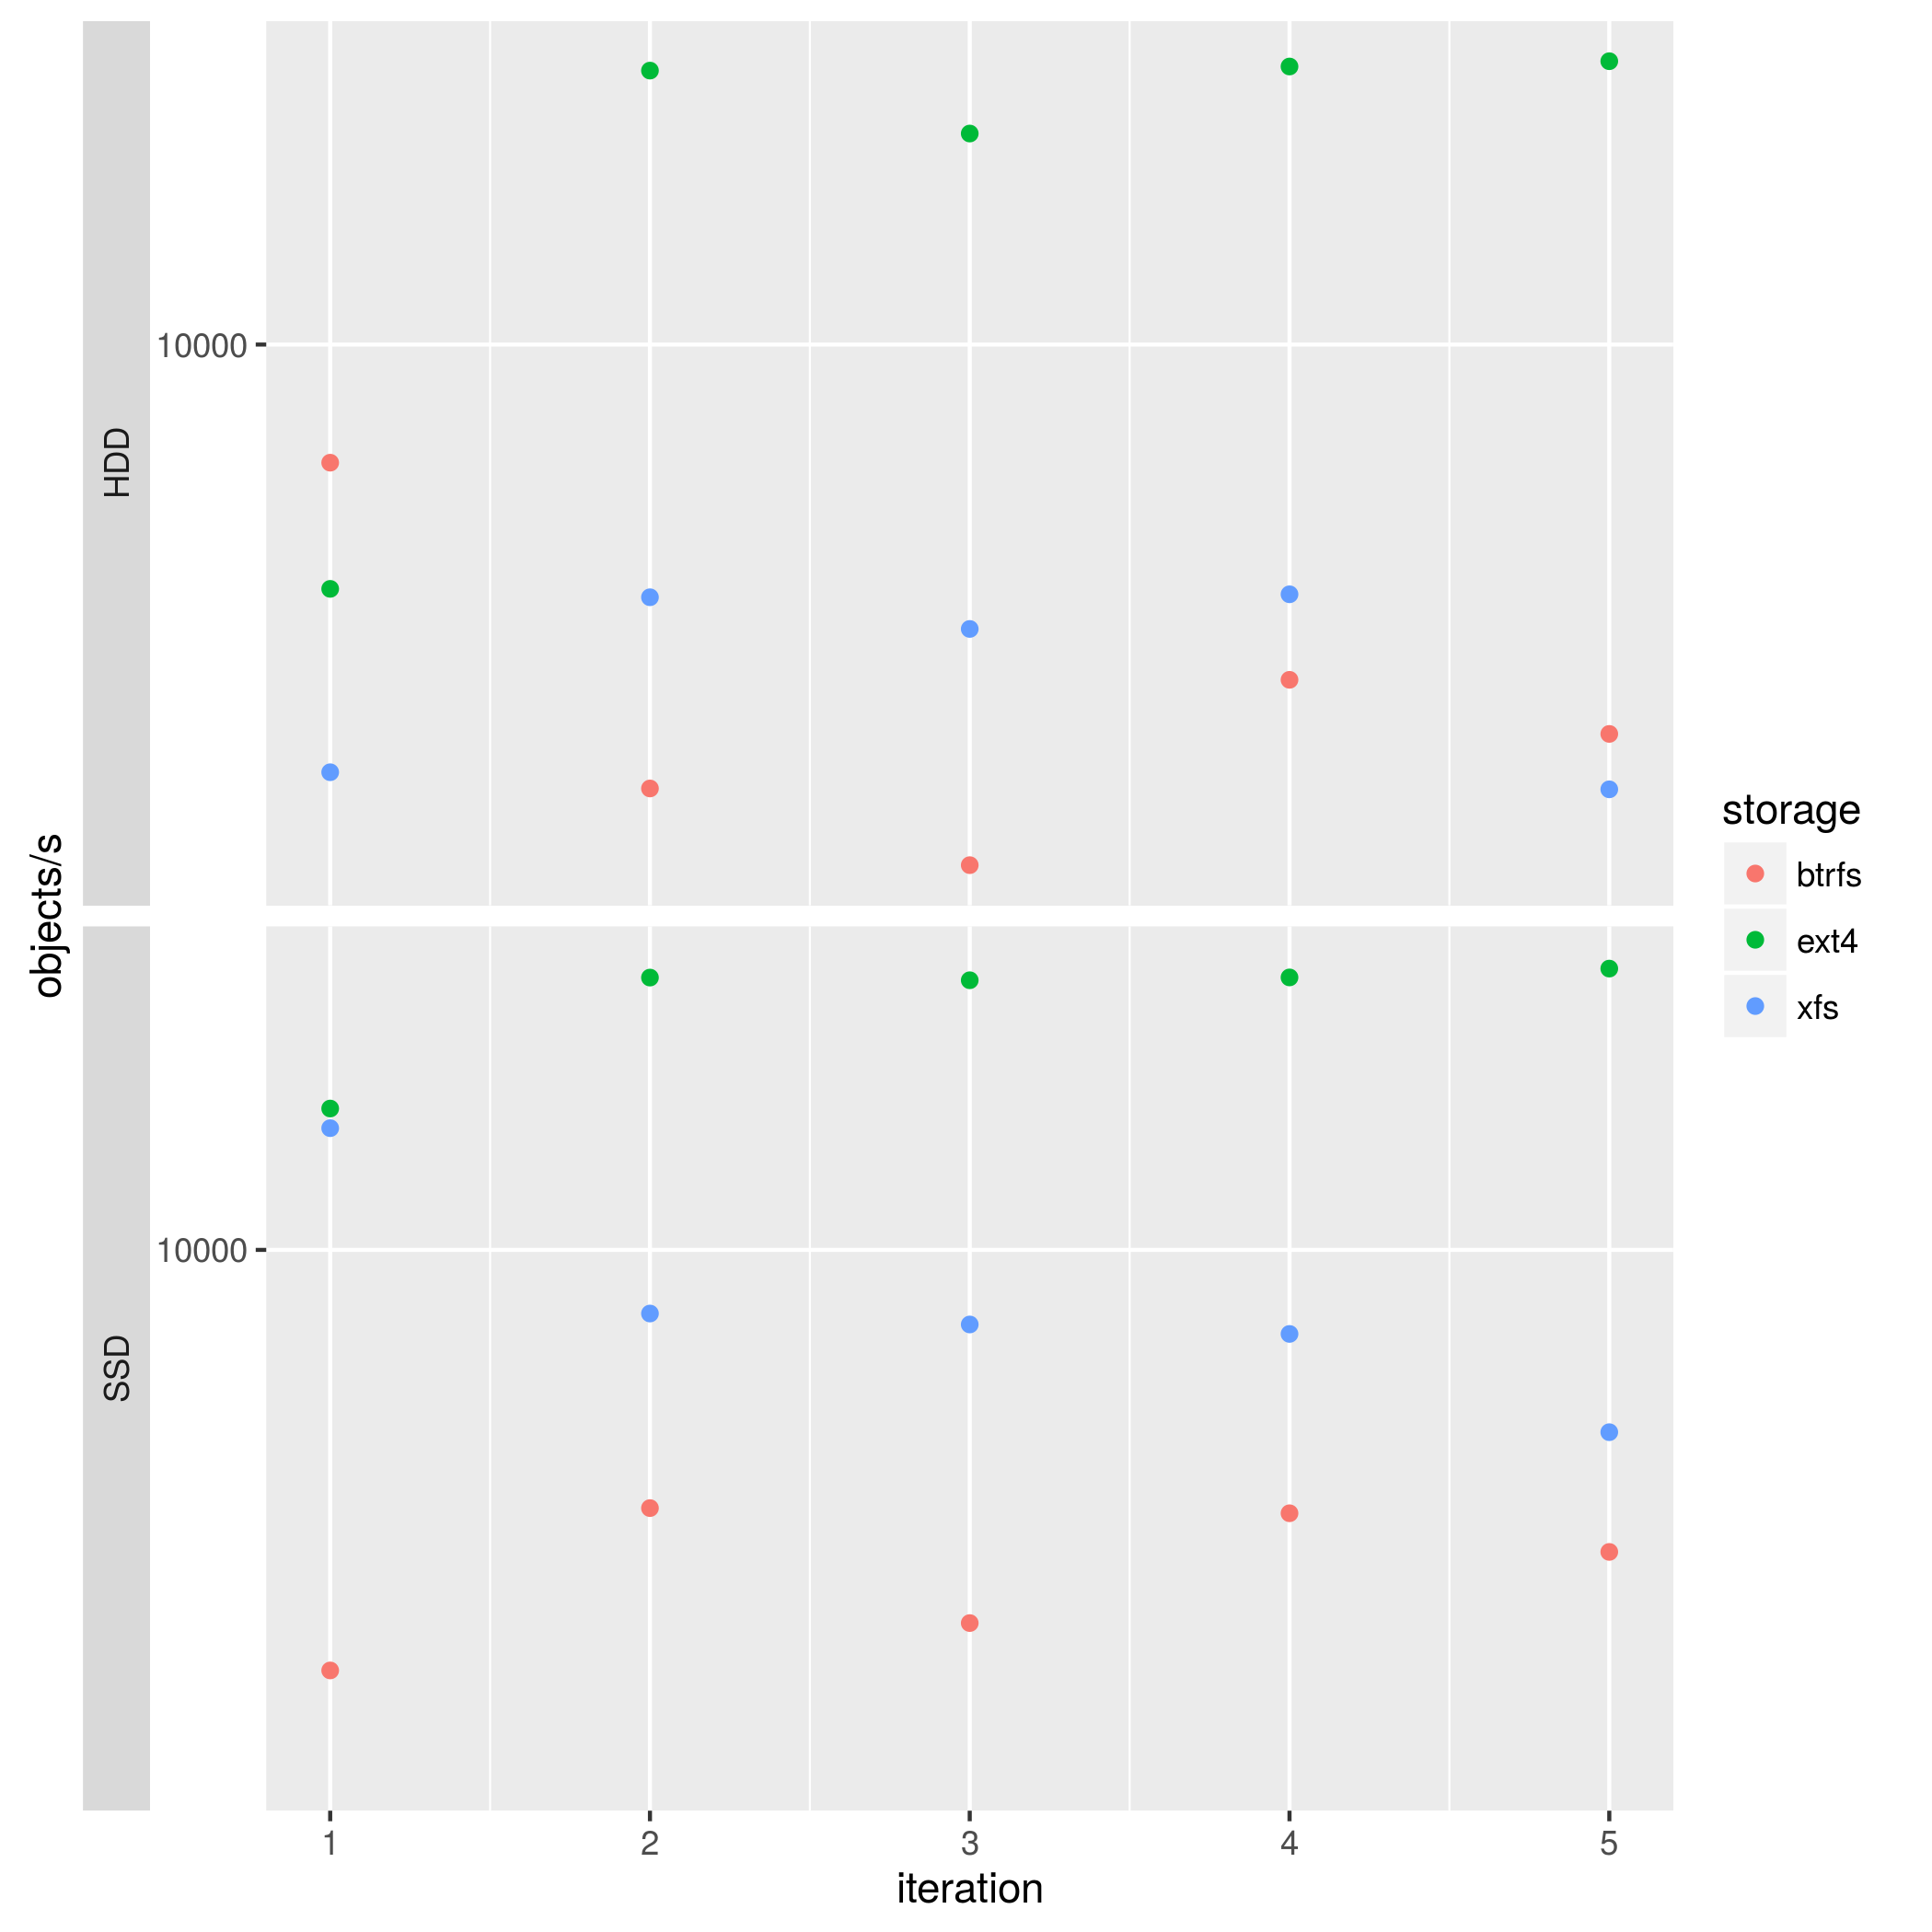
\includegraphics[width=8cm]{10tp-fs}}
\subfloat[2 processes]{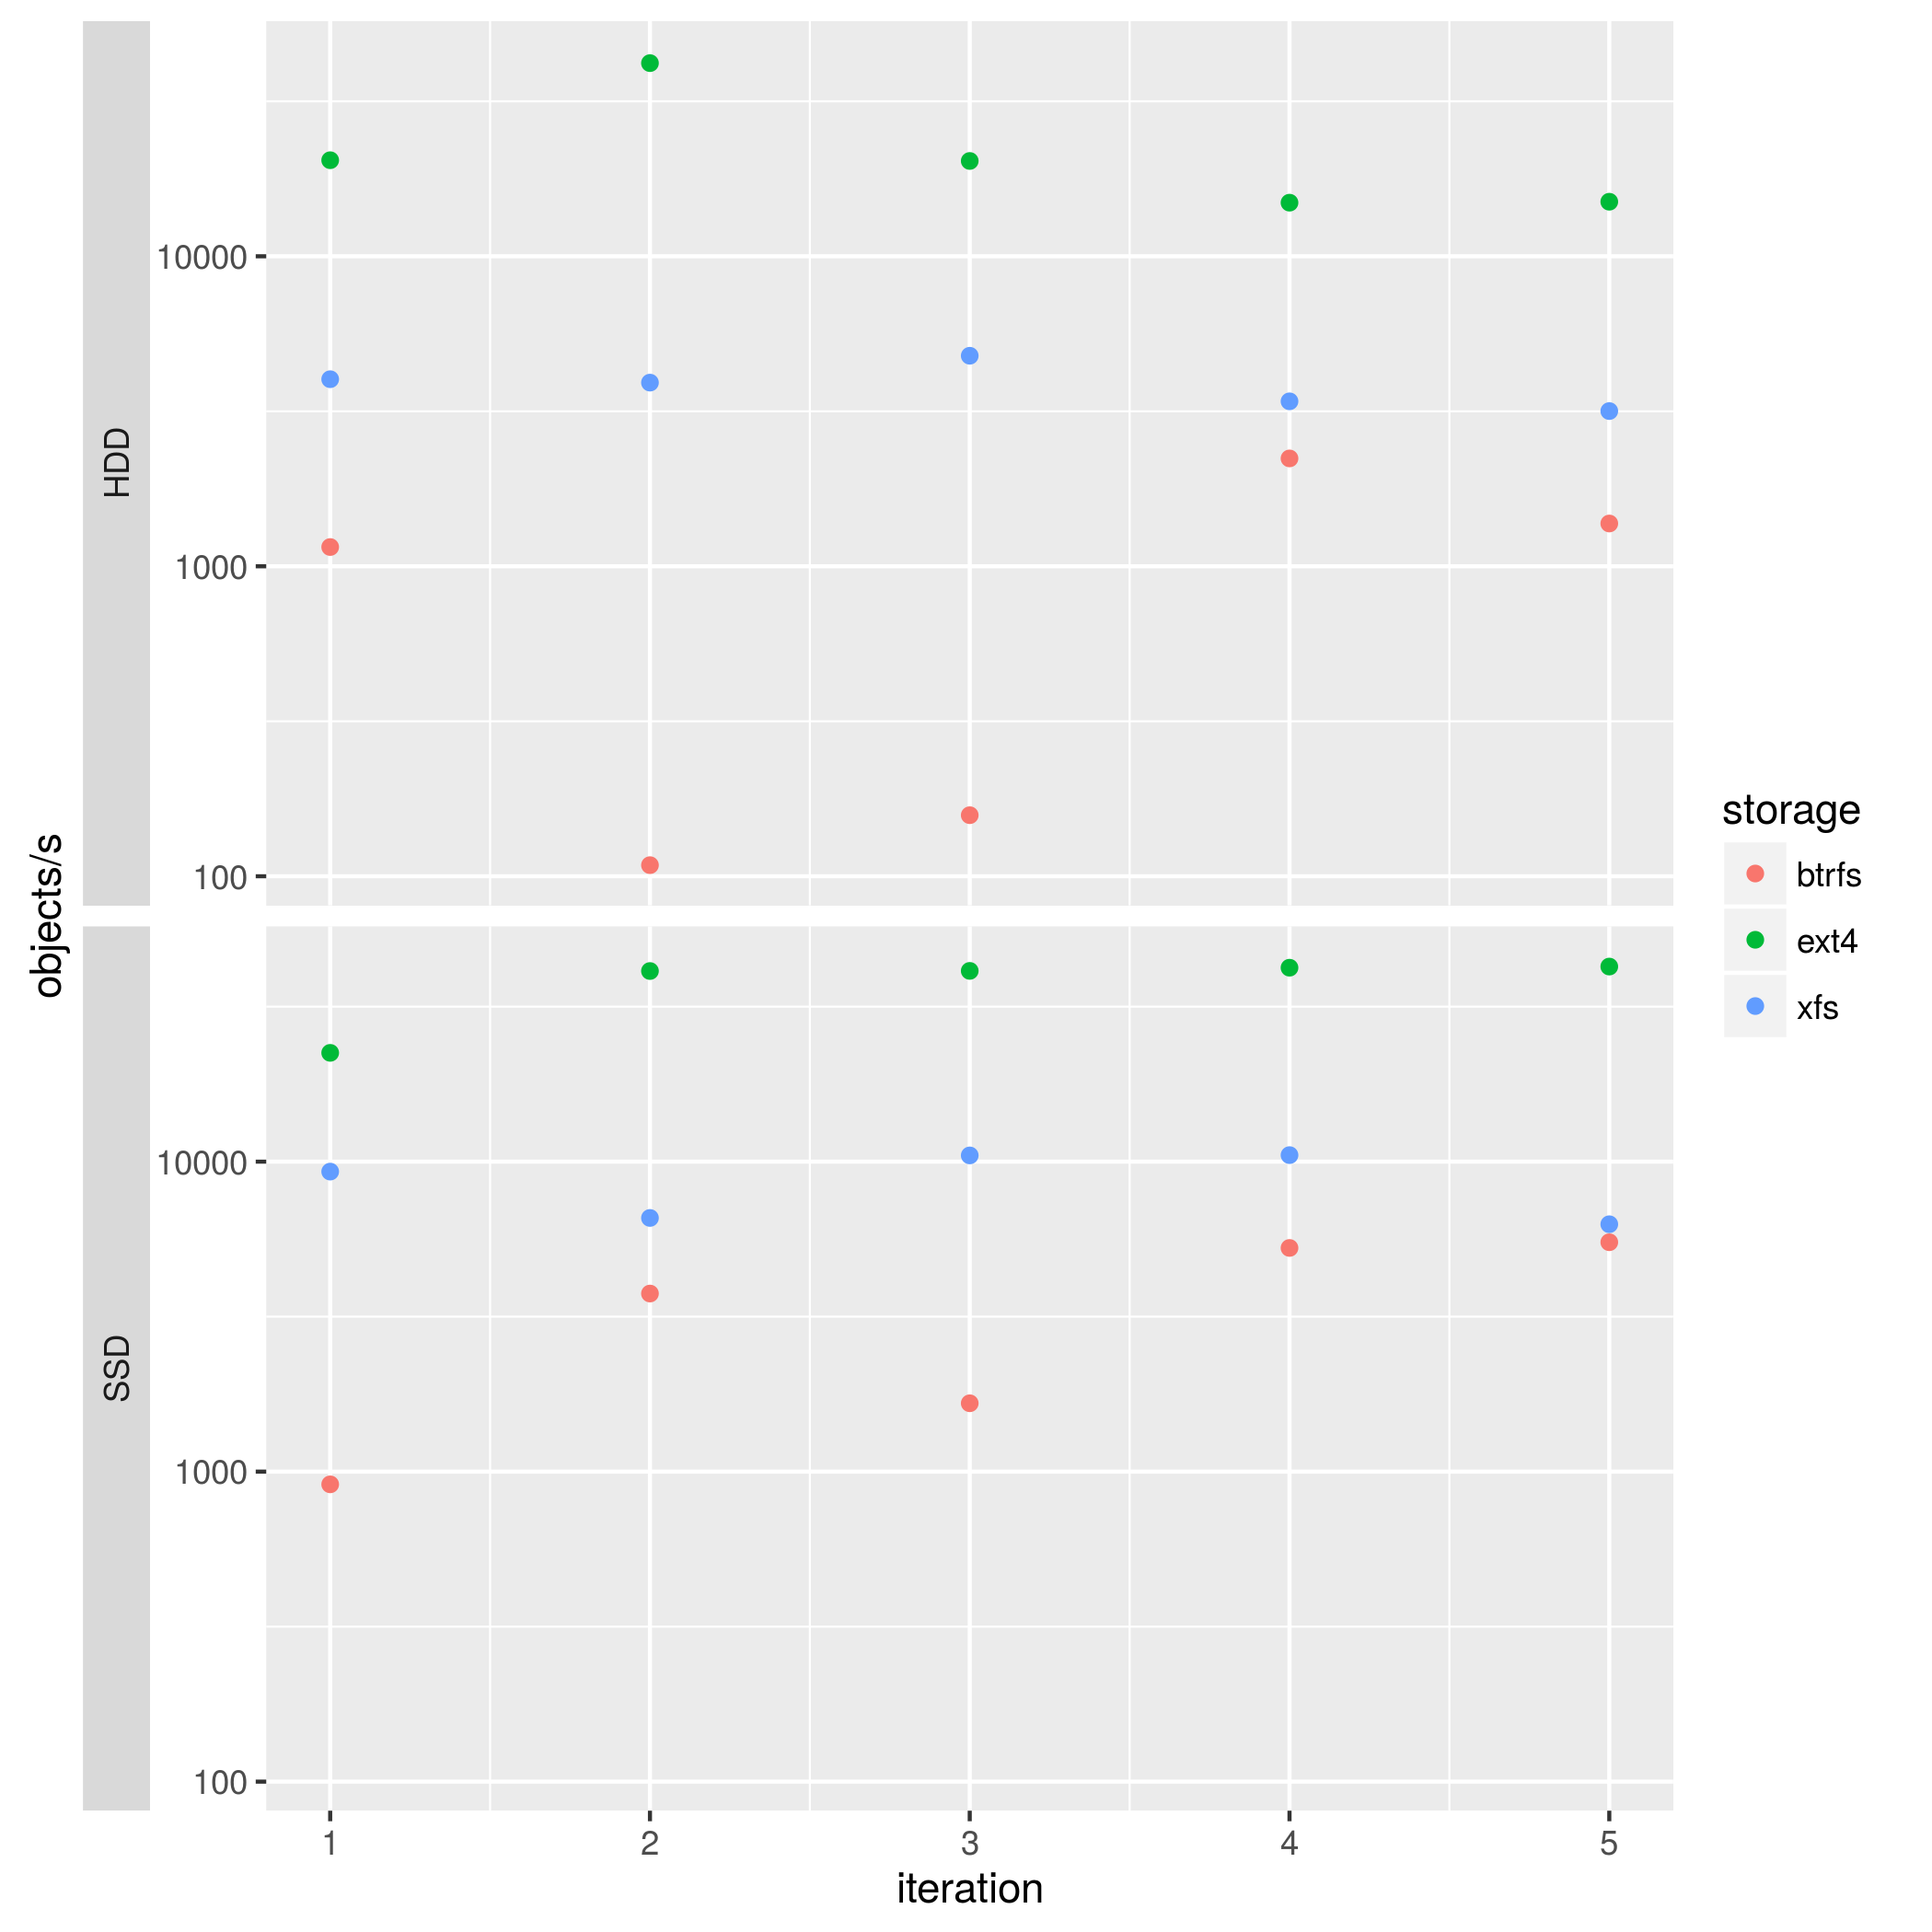
\includegraphics[width=8cm]{10tp-2proc-fs}}
\caption{Variability between the repeated runs. \label{fig:10variability}}
\end{figure}


\section{Summary}

The results demonstrate that existing file systems can optimize typical workloads rather well.
Precreate and cleanup phases follow regular patterns and are usually optimized to large I/O on HDD.
However, with sufficiently large working set exceeding the available memory, the benchmarking phase of MD-REAL-IO can reveal the capabilities of storage technology and file system.

\end{document}
